%-----------------------------------------------------------------------------
% Template for AIMS-Senegal essay phase 2011-12
%
% The fonts, linespacing, numbering, page styles, order
% of  Title/Abstract/TOC/Body/{Appendices}/Acknowledgements/References 
% are prescribed as the AIMS house style.
%
% Do not change them or add to it without getting approval first.
% Essays are not accepted if they do not follow house style.
% This is in preparation for your Masters/PhD where the university
% will be much more strict on the house style.
%
\documentclass{aimsessay}
%
%-----------------------------------------------------------------------------
% To use external packages for specific needs, 
% get approval before adding them here (they
% should not override general AIMS house style and layout).
%
% Examples:
%
% For tables:
\usepackage{booktabs} % \toprule, \midrule, \bottomrule
\usepackage{array}    % \newcolumntype
% 
% For figures:
\usepackage[below]{placeins} % use \FloatBarrier in the body
% \usepackage{float}  %"H" placement spec, for **really here** (i.e. not float)
% \usepackage{subfig} %many figures in one figure (note subfigure is deprecated)
%
% For code and algorithms
\usepackage{moreverb}   % \verbatimtabinput
% For links and hyper references
\usepackage{hyperref}
\urlstyle{same}
% \usepackage{listings} % more flexible and complicated 
                        % than moreverb and algorithm
% To include accented French Characters
\usepackage[french]{babel}
\usepackage{ucs}
\usepackage[utf8x]{inputenc} 
% To change the Interface Language
%Options > Interface Language > choose "en" or "fr"
% then restart Texmaker.
% Others
% \usepackage[all]{xy} 
% \usepackage{sagetex}
% \usepackage{siunitx} % to typeset numbers, units, align decimals in tables.
% \usepackage{dcolumn} % less flexible but maybe faster than siunitx above.
% \usepackage{mathtools} % More maths, e.g. \mathclap.
%
% Others may be landscape, longtable, algorithm, algorithmic, etc.
% 
% ----------------------------------------------------------------------------
% An AIMS Essay can use the sectioning commands "\chapter", "\section",
% "\subsection". No "\subsubsection", "\paragraph", etc. They are disabled.
% 
% For Theorems and such, use the environments defined here:
% \begin{thm}...\end{thm} (or "lem", "defn", etc)
% 
% We put the number to the left of the Theorem heading.
\swapnumbers 
% 
% Theorems are in italics.
\theoremstyle{plain}
\newtheorem{thm}[subsection]{Theorem}
%
% Rest is not in italics.
\theoremstyle{definition} 
\newtheorem{lem}[subsection]{Lemma}
\newtheorem{cor}[subsection]{Corollary}
\newtheorem{conj}[subsection]{Conjecture}
\newtheorem{pro}[subsection]{Proposition}
\newtheorem{exa}[subsection]{Example}
\newtheorem{defn}[subsection]{Definition}
\newtheorem{rem}[subsection]{Remark}
% 
% If you have no theorems, but a lot of equations, maybe the
% following two lines are good. Beware of corresponding Equation
% and Example numbers though! Number equations by sections.
% 
\numberwithin{equation}{section}
% 
%-----------------------------------------------------------------------------
% Abstracts are usually written in English, with a version in your
% mother tongue underneath.
%
% French, Igbo, Malagasy, etc. students use normal latex
% for special characters, for example \'{e}
%
% Amharic students use openoffice to write Amharic,
% export and include a figure.
%
% Arabic students uncomment this line to write your abstract, 
% and see the example below:
%\usepackage{arabtex}                         
%\usepackage{utf8} 
%\setcode{utf8}    
% Then in the MAIN BODY use this:                  
%% \begin{RLtext}    
%% Here is where the arabic text goes.
%% You can just type it with an arabic keyboard
%% \end{RLtext}
%-----------------------------------------------------------------------------
% Your own command shortcuts can go here
% keep them clearly separate from other sections of the preamble
% It is good style to have only a few of these so that
% we can read one another's code. If you have to many, 
% then your code does not compile in someone else's template easily,
% and it makes it harder to read. These definitions are only
% meant for very often-used commands to save typing; Examples:
%
%\newcommand {\be}{\begin{equation}}
%\newcommand {\ee}{\end{equation}}
%\newcommand {\C}{\mathbb{C}} % Complex
%\newcommand {\Z}{\mathbb{Z}} % Integers
%\newcommand {\R}{\mathbb{R}} % Real
%\DeclareMathOperator{\sech}{sech} % declaring new math operators like \sin.
%  
%-----------------------------------------------------------------------------
% Title & Author
% On this page you must have NO full-word capitalizations, bold, or colour. 
% All AIMS essays per year have the same title page.
% In English your family name is written last, and with 
% English Capitalization, not as in some Francophone countries where
% you write LASTNAME, Firstname.
% Put your AIMS email address only please, for consistency,
% not gmail or some other webmail address.
\title{The Essay Title goes here}
% Your name must be in English Capitalisation with no comma, 
% and the Family name comes last.
\author{Firstname Middlename Familyname (email@aims-senegal.org)\\
% Igbo, French students, put your special characters above.
% Arabic students can add their name in Arabic letters below, 
% after the english one
% Uncomment the next four lines and edit the name
%%%%%%%%%%%%%%%%%%%%%%%%%%%%%%%%%%%
%\begin{RLtext}
% شةشىغ
%\end{RLtext}
%%%%%%%%%%%%%%%%%%%%%%%%%%%%%%%%%%%%%
% Amharic students speak to me about how to add your name in your own alphabet.
% Everything here is prescribed; do not enter bold or ALL CAPS here,
% it will not be accepted.
L'Institut Africain des Sciences Mathématiques (AIMS)\\
Sénégal\\\\
% Example1
% Supervised by Professor Barry Green
% University of Stellenbosch, South Africa
% Example2
% Supervised by Doctor Ingrid Rewitzk
% University of Stellenbosch, South Africa
{\small Supervisé par: Title Firstname Lastname}\\
{\small Institute of Supervisor, Country}%
% Don't put the department, it becomes too long.
}
\date{{\small 19 Mai 2016}\\%
  {\scriptsize\it Présenté pour Realisation Partielle d'un Master II à AIMS}\\%
  \vspace{3cm}{
\includegraphics[width = 12cm]{images/aimssn-logo.jpg}}}
%-------------------------------------------------------------------------
\begin{document}
\pagestyle{empty}
\maketitle
% All other files are included via \input. 
% To compile in texmaker while viewing any of those
% without having to switch back, use
%   Options > Define Current Document as 'Master Document'
% To not have to close a PDF, remove viewpdf from quickbuild 
% and open the PDF (once) manually: it will auto-refresh or with control-r
% 
%-------------------------------------------------------------------------
% The abstract is the first thing we want to see. No acknowledgements or 
% dedications here. Fetch the abstract from a separate file.
% Please write it in English and in your mother tongue.
% An abstract should be less than half a page, so that both abstracts 
% (that is both languages) fit onto one page.
% We number roman numerals until the main body
\pagenumbering{roman}
% Abstracts are usually written in English, with a version in your
% mother tongue underneath
\chapter*{Abstract} 
\addcontentsline{toc}{chapter}{Abstract}
% Don't change anything above this.

A short, abstracted description of your essay goes here. 
It should be about 100 words long. But write it last.

An abstract is not a summary of your essay: it's an abstraction of that. 
It tells the readers why they should be interested in your essay but summarises all
they need to know if they read no further.

The writing style used in an abstract is like the style used in the rest of your essay: concise, clear and direct. 
In the rest of the essay, however, you will introduce and use technical terms. In the abstract you should
avoid them in order to make the result comprehensible to all.

You may like to repeat the abstract in your mother tongue.

% At a unviersity like Stellenbosch you *must* produce an abstract in Afrikaans for your masters.
% At AIMS you are encouraged to repeat the abstract in your mother tongue
% French, Igbo, Mlagasy, etc. just write it using LaTeX's special
% characters.
% Arabic students use the arabtex package.
% Amharic use openoffice and export from there and import a figure here.
% Where the words do not exist put the English work in italics, or use mathematical symbols.


% Do not change anything below this except for adding your
% signature and name. And take the message to heart.
\vfill
\section*{Declaration}
I, the undersigned, hereby declare that the work contained in this essay is my original work,
and that any work done by others or by myself previously has been 
acknowledged and referenced accordingly.

% Scan your signature into a small picture called 'signature.png' and insert it
% above your name and the date:
%\includegraphics[height=2cm]{signature.png} \newline \hrule
% Your name must be in English Capitalisation with no comma, and the Family name comes last. 
% Do note the date below. It is called the "deadline".
Firstname Middlename Lastname, 15 May 2014

% Don't go typing out the contents.
\tableofcontents
% We strongly *discourage* lists of figures, glossaries, and indices 
% under the AIMS essay style. Get approval before uncommenting this. There
% has to be a good reason for your essay to be navigable in this form, e.g.
% an abnormally large number of figures, or a graphically oriented topic
%\listoffigures
%\addcontentsline{toc}{chapter}{List of Figures}
%-----------------------------------------------------------------------------
\newpage
% We switch to arabic numerals here where your page count starts
% Essays must be 25-30 pages long *starting here* and up to and including
% the conlcusion. It does not include the acknowledgements or references.
% 
% Figures may differ between topics, but they are not there
% to fill the pages -- they must add meaning.
% In general most figures should be 0.8 times the width of the page
% (perhaps wider when two or three columns of figures)
% See the example in chapter one for defining that. B1e *consistent*
% in your presentation of information.
\pagenumbering{arabic}
\pagestyle{myheadings}
%-----------------------------------------------------------------------------
% Each chapter goes in a separate file
% Chapter titles are just examples
% Always have a question
% Note the Case Pattern used at AIMS

\chapter*{Introduction}
\label{chp: chap1}
 


 % Introduction is usually a chapter itself.
\chapter{Preliminary} 
\section{Motivation and Context}
The last decade has witnessed real progress in the geophysical research area. This fact is due to the development of new approach in seismic modeling such as Full Waveform Inversion (FWI), and the opportunity that offers the High Performance Computing (HPC). The rapid increasing of the HPC technologies allows to deal with large test cases with significant performance. In this insight, a group of researcher working in Geoazur laboratory and Observatory of C\^{o}te d'Azur (OCA) has developed advanced seismic imaging methods. To share the benefit of their work in the scientific community, they make in open-source distribution many of their packages. At the same time, These researchers are involved the SEISCOPE consortium sponsored by 9 companies Gas and Oil (see http://seiscope2.osug.fr) from which their work is promoted. 

In this perspective, the SEISCOPE team has developed an efficient code for full waveform inversion, called DSFDM/FFWI (Direct Solver Finite Difference Method / Frequency FWI). The DSFDM/FFWI code was applied successfully in real seismic dataset collected in ocean-bottom cable data from the Valhall oil field (North Sea) in the visco-acoustic vertical transverse isotropic (VTI) approximation \cite{}. For its running, this code uses different packages especially MUMPS (MULtifrontal Massively Parallel sparse direct Solver) to solve the wave propagation equation with direct-solver method which is the most expensive part of the inversion process. 

The modelling in a frequency domain is a promising method because it naturally takes into account the attenuation, a physical characteristic that can greatly impact the seismic imaging quality in certain cases,  but also because of its speed of calculation for simulations with multiple right-hand side. The backwards of this method, which has prevented its expansion rapidly, is its memory consumption which limits it to medium-sized use cases.

Bull, a company of Atos group, has developed its second generation of server x86 with large shared memory, called MESCA-II (Multiple Environments on a Scalable Csi-based Architecture. Technically, a Mesca node can have 8 sockets    
....

\section{Geophysical Seismic Imaging}
\subsection{Introduction}
 
The Earth is characterised by seismic activities. Human has been always animated by the curiosity to understand these activities. During years, human used different techniques to explore the basement depths. Recently, this exploration is more motivated by multiples reasons that can be economics, social, environment, scientific etc. For instance, the study of the nature the soil is useful fol civil engineers, landslide imaging is very useful for estimating the risk of gravity, the detection of oil and mineral resources present a major economic challenge, the monitoring of radioactive waste landfill areas or CO2 injection represents an new environmental challenge.  

With the advents of Industrial revolution accompanied by the higher need to find new oilfield by hydrocarbon industry, the seismic imaging technique has successfully used from the mid of 19th. By definition, Seismic imaging is a tool that bounces sound waves off underground rock structures to reveal the possible tectonic structures []. In seismic modelling, one need data coming from seismic wave propagation to create good quality images of the subsurface (imaged by acoustic waves). The acoustic waves are generated under the Earth by sources that can be man-made devices or by earthquakes. Receivers or seismometers acquire information that can provide details of the velocity and the geometric structure of the Earth. 


During years scientists invent several techniques of seismic imaging which include Electrical Resistivity Tomography,  Ground penetrating radar, Induced polarization and Seismic Tomography and Reflection seismology.
\begin{itemize}
\item \textbf{Electrical Resistivity Tomography (ERT)}. The ERT technique is invented by Schlumberger brothers and developed by the work of Andrey Nikolayevich Tikhonov []. This method is an electrical testing method where electrical current is induced in the ground between one pair of electrodes and the voltage is measured between another pair. These measurements are used to estimate lateral and vertical variations of resistivity values of the earth. ERT can be used to map geologic variations (soil lithology, presence of ground water, fracture zones, variations in soil saturation, areas of increased salinity or, in some cases, ground water contamination), bedrock depths and geometry, mapping cavities such as caves, karst and/or evaporite dissolution sinkholes. Like other seismic technique, ERT has the capacity to yield either 1D (sounding), 2D (profile) or 3D (volume) imaging.  

\item \textbf{Ground Penetrating Radar (GPR)}. GPR systems work by sending a tiny pulse of energy into a material via an antenna. An integrated computer records the strength and time required for the return of any reflected signals. Subsurface variations will create reflections that are picked up by the system and stored on digital media []. This technique has many applications: civil engineering, resources explorations.  

\item \textbf{Induced Polarization (IP)}. Similar to electrical resistivity tomography, this technique measure the electrical chargeability of subsurface materials. IP provide additional information about the spatial variation in lithology and grain-surface chemistry. It can be made in time-domain and in frequency-domain.  IP method is widely used in mineral exploration and mining industry and it has other applications in hydrogeophysical surveys, environmental investigations and geotechnical engineering projects.
 
\item \textbf{Reflection Seismology (RF)}. This is the most wide used technique when we talk about hydrocarbon exploration, or mineral exploration. RF is a form of echo sounding, detecting echoes from seismic interfaces. It can yield results that are the closest of any geophysical technique to a conventional geological section. The waves propagation under the Earth require to know some features of the wave: transmission, absorption, and attenuation in the earth materials and its reflection, refraction, and diffraction characteristics
at discontinuities.   

In the context of onshore, geophysicists use geophones as receivers to collect the speeds of particles on the ground. Accelerometer sensors can be used to record these data. These sensors are directional and measure the speed or acceleration in a spatial direction. Sometimes, devices with multi-components are used to measure wavefields in the horizontal directions (parallel to the Earth's surface) and vertical direction, thus identifying the different types of waves whose depend on the directions []. The figure \ref{geophones} shows the scenario of ....  

\begin{figure}[!h]
% Use "\centering" in floats (figure, table), but if you need to center
% some text (why?) use "\begin{center}...\end{center}".
\centering 
% Figure environments same as 0.8 * \textwidth please
% That does not necessarily mean the actual picture size,
% it is a guideline for the environment which could contain
% 2 or more pictures! Be consistent and follow the guidelines
% provided in your sources.
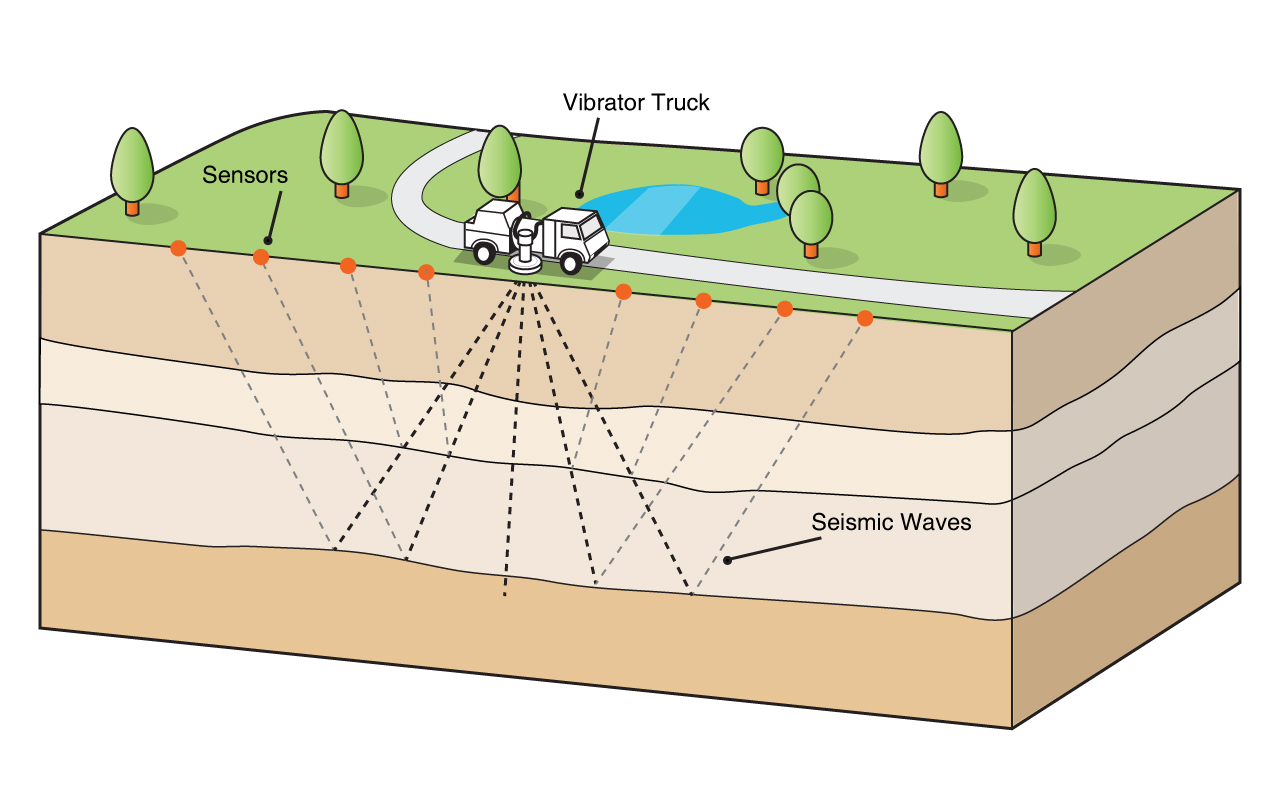
\includegraphics[width=0.6\textwidth]{images/geophones.jpg}
\caption{Seismic imaging.}
\label{geophones} 
% if you move the label it breaks the reference numbering; 
% always have it *after* the caption.
\end{figure}

In the off-shoring scenario, the hydrophones, placed on the surface of the sea, are often used to collect the seismic wavefields information. In the figure \ref{hydrophones}, a ship generates the seismic source by an air gun and drag behind, under the water surface, a raw of hydrophones measuring the pressure field which indicates the waves propagated in the structure of the subsoil. Others sensors named \textit{Ocean Bottom Seismometer} (OBS) are designed to record the earth motion under oceans and lakes from man-made sources. These devices can stay several days under the water. Each OBS receives different acoustic waves for each generation of sound arriving at different times. There exists another device called Ocean Bottom Cable (OBC).The data acquisition is performed by multi-component sensors bound on the cables. 
\begin{figure}[!h]
% Use "\centering" in floats (figure, table), but if you need to center
% some text (why?) use "\begin{center}...\end{center}".
\centering 
% Figure environments same as 0.8 * \textwidth please
% That does not necessarily mean the actual picture size,
% it is a guideline for the environment which could contain
% 2 or more pictures! Be consistent and follow the guidelines
% provided in your sources.
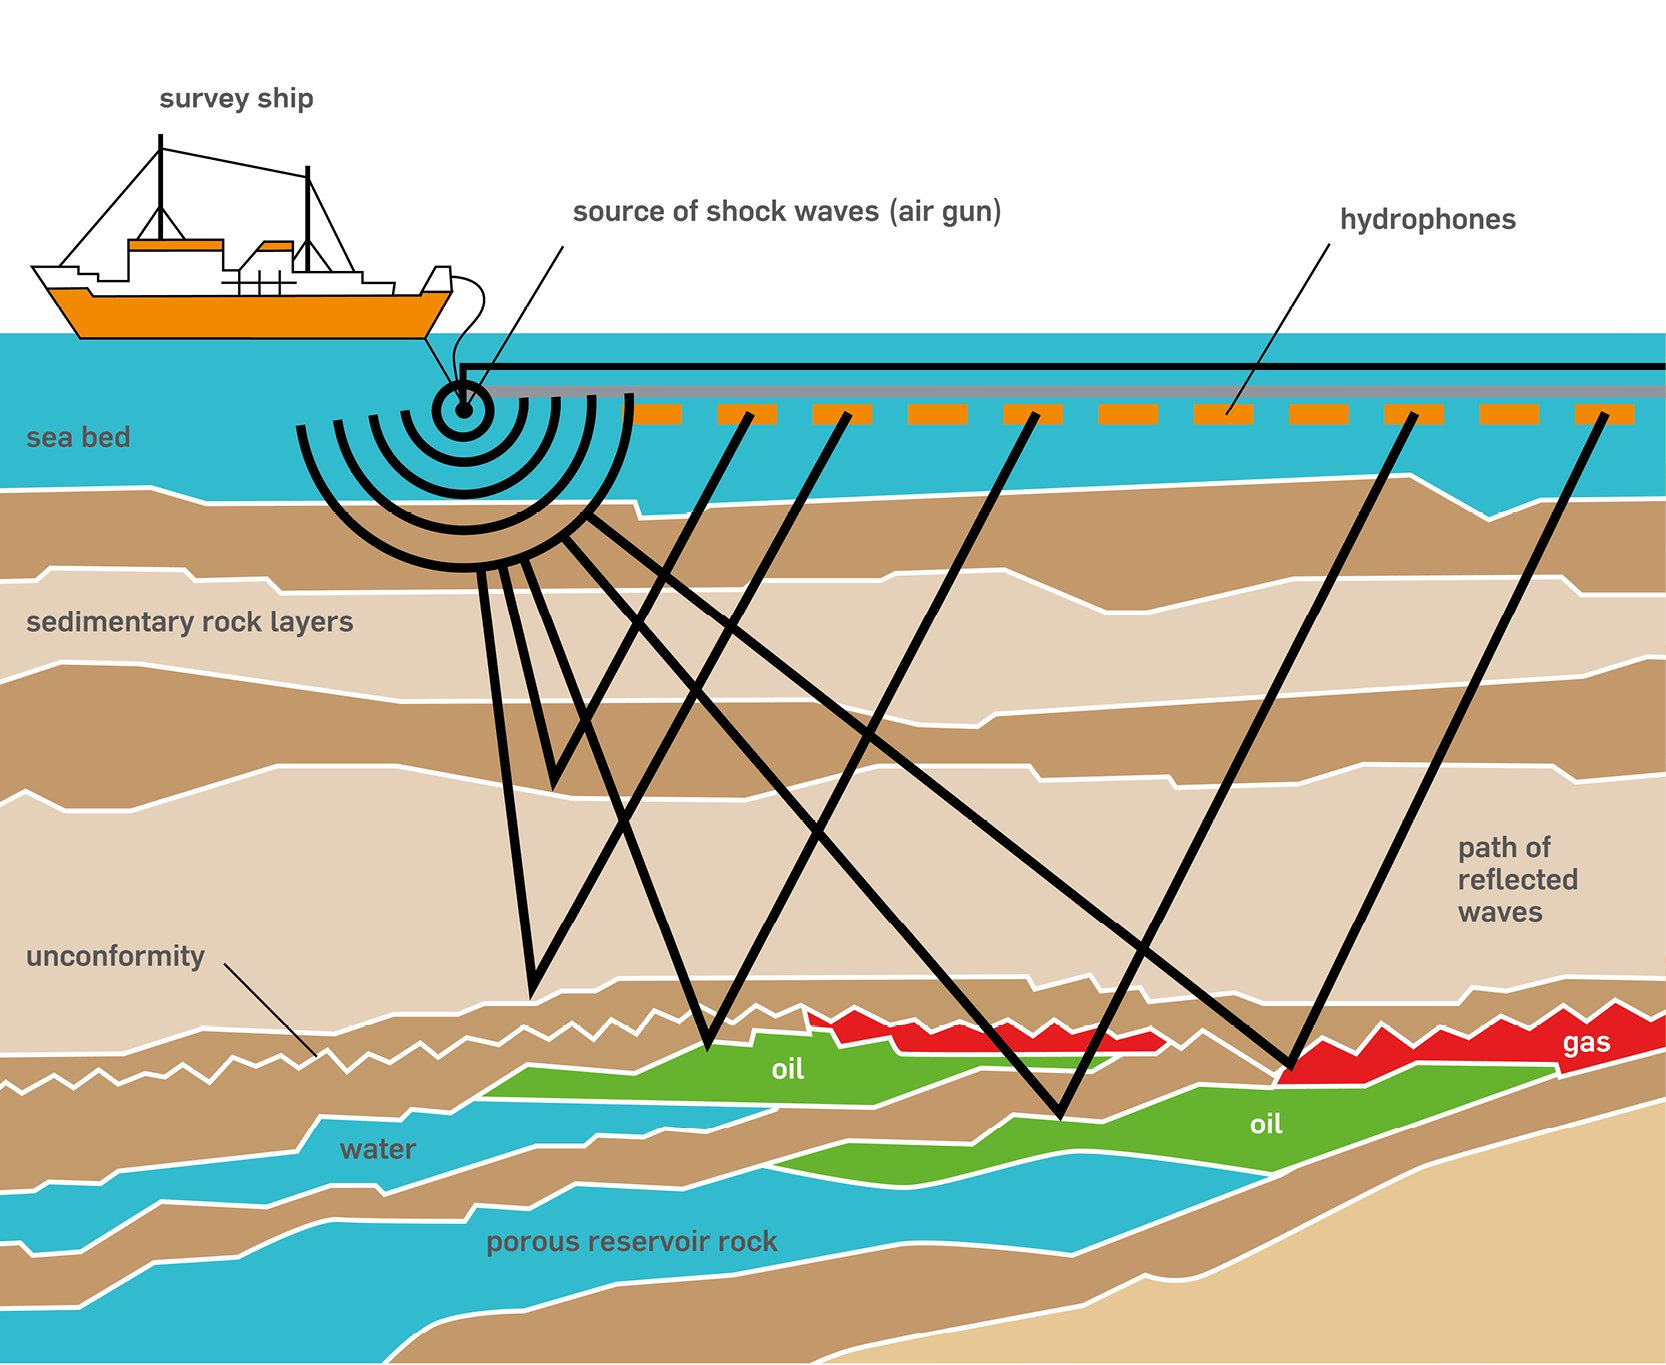
\includegraphics[width=0.6\textwidth]{images/hydrophones.jpg}
\caption{Seismic imaging.}
\label{hydrophones} 
% if you move the label it breaks the reference numbering; 
% always have it *after* the caption.
\end{figure}
\end{itemize}

\subsection{Seismic model}
These techniques need numerical methods to solve the seismic imaging problem. In this study, we just focus on Frequency-domain seismic modeling based on the sparse direct solver (DSFDM)and Full Wave Inversion method used by Seiscope Consortium to develop the DSFDM/FWI code.

The DSFDM is a finite-difference frequency-domain method, which has aimed to solve linear systems resulting from the discretization of the time-harmonic wave equation with sparse direct solvers. This method with 27 stencils has developed in a visco-accoustic vertical transverse isotropic (VTI) [Operto et al. (2007), Brossier et al. (2010), Operto et al. (2009) and Operto et al. (2014)]. It is governed by the linear systems resulting by 3D visco-acoustic VTI wave equation:
\begin{align}
Ap_h &= b   \label{eq1}\\
p_v &= Bp_h + s^{'}, \label{eq2}\\
p &= (2p_h + p_v)/3 \label{eq3}
\end{align}
where the matrices $ A $ and $ B $ result from the discretization of operators.

\begin{align}
A &= \omega^{2} \left[ \frac{\omega^{2}}{\kappa_{0}} + (1+2 \epsilon) (\mathcal{X} + \mathcal{Y}) + \sqrt{1+2\delta} \mathcal{Z} \frac{1}{\sqrt{1+2\delta}} \right] \label{eq4}\\
B &= \frac{1}{\sqrt{1+2\delta}} + \frac{2(\epsilon - \delta)\kappa_{0}}{\omega^{2}\sqrt{1+2\delta}} (\mathcal{X} + \mathcal{Y}) 
\end{align}

Similarly, the source terms are given by:

\begin{align}
b &= \frac{\omega^{4}s_{h}}{\kappa_{0}} s - \omega^{2}\sqrt{1+2\delta} \mathcal{Z} \left(s_{v} - \frac{1}{\sqrt{1+2\delta}}s_{h} \right)s, \label{eqb}\\
s^{'} &=  \left(s_{v} - \frac{1}{\sqrt{1+2\delta}}s_{h} \right)s
\end{align}

The wavefields $ p_h = \sigma_{xx} = \sigma_{yy} $ and $ p_v = \sigma_{zz} $ are the so-called horizontal and vertical pressure wavefields, respectively (Plessix and Cao, 2011). The angular frequency is denoted by $ \omega$, $ \kappa_{0} = \rho V_{0}^{2} $  where $ \rho $ is the density and $ V_0 $ is the vertical wavespeed, $ \delta $ and $ \epsilon $ are the Thomsen's parameters. The seismic source vector is compactly denoted by $ s $. For an explosion and vertical force, the expression of the source vector is given by 
\begin{align}
s_{explosion} &= s(\omega) \hat{\delta}(x_s - x) \\
s_{vertical_force} &= s(\omega)d_z \hat{\delta}(x_s - x) 
\end{align}

where $s(\omega)$ denotes the Fourier coefficient of the temporal source wavelet for the modeled frequency, $d_z$ the derivative with respect to $z$,$\hat{\delta}$ the delta function, $x_s$ the coordinates of the source position. 

The $s_h$ and the $s_v$terms are given by the following formulas.
\begin{align}
s_h &= (2(2+\epsilon)+ \sqrt{1+2\delta})/D, \\
s_v &= (1+2\sqrt{1+2\delta})/D, \\
D &=  4\sqrt{1+2\epsilon} + 4 \sqrt{1+2\delta} + 1
\end{align}
The expression of $ D $ was corrected relative to the one provided in Operto et al. (2014). \newline
The second-order differential operators $  \mathcal{X}$ , $ \mathcal{Y}$ and $ \mathcal{Z}$ are given by
$$ \mathcal{X} = \partial_{\tilde{x}} b  \partial_{\tilde{x}},  \mathcal{Y} = \partial_{\tilde{y}} b  \partial_{\tilde{y}},  \mathcal{Z} = \partial_{\tilde{z}} b  \partial_{\tilde{z}},  $$

where $b=1/\rho$ is the buoyancy and the complex-valued coordinate system $(\tilde{x}, \tilde{y}, \tilde{z})$ is used to implement perfectly-matched layers absorbing boundary conditions (Bérenger, 1994; Operto et al., 2007).
If we assume that $\delta$ is slowly varying and hence can be considered as locally homogeneous, the operator $ A $ can be simplified as
\begin{equation}
A_{a} = \omega^{2} \left[ \frac{\omega^{2}}{\kappa_{0}} + (1+2 \epsilon) (\mathcal{X} + \mathcal{Y}) + \mathcal{Z} \right] 2 \mathcal{Z}\kappa_{0} (\epsilon - \delta)  (\mathcal{X} + \mathcal{Y}) \label{eq13}
\end{equation}
In this case, the wave operator within the bracket describes wave propagation in an elliptic medium,
while the second term accounts for anellipticity.

In \textit{elliptic} media $ (\delta=\epsilon \neq 0 ) $, the source become

\begin{align}
b &= \frac{\omega^{4} s_h}{\kappa_{0}} s \\
s^{'} &= 0
\end{align}

The authors mention  this point because the second term of the source $b$, equation \ref{eqb}, involves a second-order vertical derivative which can be tricky to implement if the source does not match the grid point. Therefore, it is worth assuming that the medium is elliptic at the source positions if this is a reasonable assumption.

In isotropic media $(\delta = \epsilon = 0)$, one can easily check that Equations \ref{eq1}-\ref{eq3} reduces to
\begin{equation}
\left[ \frac{\omega^{2}}{\kappa} \mathcal{X} + \mathcal{Y} + \mathcal{Z} \right] p=\frac{\omega^{2}}{\kappa} s \label{eq16}
\end{equation}

where the operator $\left[ \frac{\omega^{2}}{\kappa} \mathcal{X} + \mathcal{Y} + \mathcal{Z} \right]$ represents the operator $A_{iso}$

Similarly, the operator $A$ can be rewritten considering the NMO velocity $(V_{NMO} = V_0\sqrt{1+2\delta} )$ in the diagonal term. This introduces the $\eta = \frac{\epsilon -\delta}{1+2\delta}$ parameter in the coefficients of the matrix.
\begin{equation}
A_{NMO} = \omega^{2} \left[ \frac{\omega^{2}}{\kappa_{NMO}} + (1+2 \eta) (\mathcal{X} + \mathcal{Y}) + \sqrt{1+2\delta} \mathcal{Z} \frac{1}{\sqrt{1+2\delta}} \right]+ 2 \sqrt{1+2\delta} \mathcal{Z} \frac{\kappa_{NMO}}{\sqrt{1+2\delta}} (\mathcal{X} + \mathcal{Y})\label{eq17}
\end{equation}
\textbf{Algorithm.} \newline
The system of three equations \ref{eq1}-\ref{eq3} is solved with the following sequence.
\begin{itemize}
\item Solve the linear system, equation \ref{eq1}, for $p_h$ with a sparse direct solver.
\item Compute explicitly $p_v$ from $p_h$, equation \ref{eq2}.
\item Compute explicitly $p$ from $p_h$ and $p_v$, equation \ref{eq3}.
\end{itemize}
The computational cost of the last two steps is negligible relative to that of the first step.

Note that wave-equation operators \ref{eq4}, \ref{eq13}, \ref{eq16} and \ref{eq17} are implemented in DSFDM code. (See Documentation)

\subsection{Full Wave Inversion (FWI)}
The Full Wave Inversion is a non linear-data fitting method that enable to get detailed estimates of subsurface properties from seismic data, which can be the result of either passive or active seismic experiments []. Basically, initialising a guess of the subsurface parameters (a model), the data are predicted from the solution of the wave propagation equation. And then, the model is always updated to minimize the misfit function between the observed and predicted data. The figure \ref{FWI} illustrates the FWI procedure. \eqref{eq1}

\begin{figure}[!h]
% Use "\centering" in floats (figure, table), but if you need to center
% some text (why?) use "\begin{center}...\end{center}".
\centering 
% Figure environments same as 0.8 * \textwidth please
% That does not necessarily mean the actual picture size,
% it is a guideline for the environment which could contain
% 2 or more pictures! Be consistent and follow the guidelines
% provided in your sources.
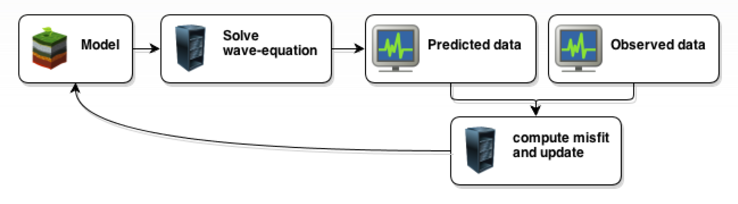
\includegraphics[width=0.8\textwidth]{images/FFWI.png}
\caption{Full Wave Inversion (FWI) procedure. from []}
\label{FWI} 
% if you move the label it breaks the reference numbering; 
% always have it *after* the caption.
\end{figure}

Mathematically, the FFWI can be formulated as an optimization problem. In [], Virieux, J. and S. Operto give the main theoretical aspects of FWI based on a least-squares local optimization approach. In a data-domain frequency-domain, FWI is an iterative reduction of the misfit function C defined as the least-squares norm of the difference between recorded and modelled monochromatic pressure data, $ d_{obs} $ and $ d(m)$, respectively.

$$ \min_{m} C(m) = \min_{m} \sum_{\omega} \Vert d_{obs} - d(m) \Vert $$

The subsurface model updated at iteration $ k + 1 $ is given by:

$$ m_{k+1} = m_{k} - \gamma_{k} \mathbf{H}_{k} \nabla_{m} C_{k} $$

where $ \mathbf{H}_{k} \nabla_{m} C_{k} $,the direction of gradient is given by the product of the gradient of C by an approximation of the inverse Hessian, H. The step length $ \gamma_{k} $ defines  quantity of descent. The descent direction can be preconditioned by a diagonal approximation of the Hessian, in our case, the diagonal elements of the so-called pseudo-Hessian matrix (Shin et al., 2001), the aim of which is to balance the gradient amplitudes with respect to depth by removing geometrical spreading effects. 

The expression of the gradient preconditioner is given by:
\begin{equation}
H = 1/ [P + \epsilon max(P)],
\end{equation}
where $P = diag \Re \left\lbrace (\frac{\partial A}{\partial m}p_h)^{\dagger}, (\frac{\partial A}{\partial m}p_h)\right\rbrace, \frac{\partial A}{\partial m}p_h$ are the so-called virtual sources  (Pratt et al., 1998) and the
damping factor $\epsilon$ should be chosen with care to balance properly in depth the gradient without generating
instabilities. For more details see Virieux, J. and S. Operto 2009, An overview of full-waveform inversion in exploration geophysics. Geophysics 74(6),.
The FFWI code is implemented with SEISCOPE optimization toolbox which contains different optimization algorithms (steepest-descent, conjugate gradient, l-BFGS, truncated Newton) including the line search [].

\subsection{Application: Valhall}
The Seismic imaging was applied in Vallhal dataset with Full Waveform Inversion method in the context of SEISCOPE project (by Operto et al.,by Operto et al.).
\begin{figure}[!h]
% Use "\centering" in floats (figure, table), but if you need to center
% some text (why?) use "\begin{center}...\end{center}".
\centering 
% Figure environments same as 0.8 * \textwidth please
% That does not necessarily mean the actual picture size,
% it is a guideline for the environment which could contain
% 2 or more pictures! Be consistent and follow the guidelines
% provided in your sources.
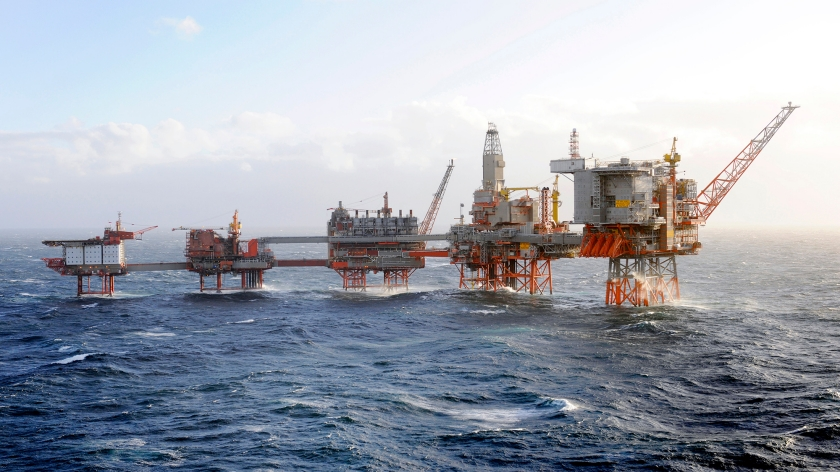
\includegraphics[width=0.6\textwidth]{images/valhall.jpg}
\caption{Full Wave Inversion (FWI) procedure. from []}
\label{valhall} 
% if you move the label it breaks the reference numbering; 
% always have it *after* the caption.
\end{figure}
The Valhall oil field is an offshore field located in North Sea in 70 m of water (see figure \ref{valhall}). In this oilfield, the presence of gas cloud is observed in the overburden. The reservoir is approximatively located in 2.5 km depth (Barkved et al. 2010). The data acquisition was making possible by wide aperture/azimuth acquisition covering a surface of 145 $km^{2}$. A layer of 12 cables contains 2302 hydrophones,
which record 49,954 explosive sources located 5 m below the surface of the water (Figure \ref{sim1}.a). A distance of 300 m separate two cables except two outer cables at 600 m. 
\begin{figure}[!h]
% Use "\centering" in floats (figure, table), but if you need to center
% some text (why?) use "\begin{center}...\end{center}".
\centering 
% Figure environments same as 0.8 * \textwidth please
% That does not necessarily mean the actual picture size,
% it is a guideline for the environment which could contain
% 2 or more pictures! Be consistent and follow the guidelines
% provided in your sources.
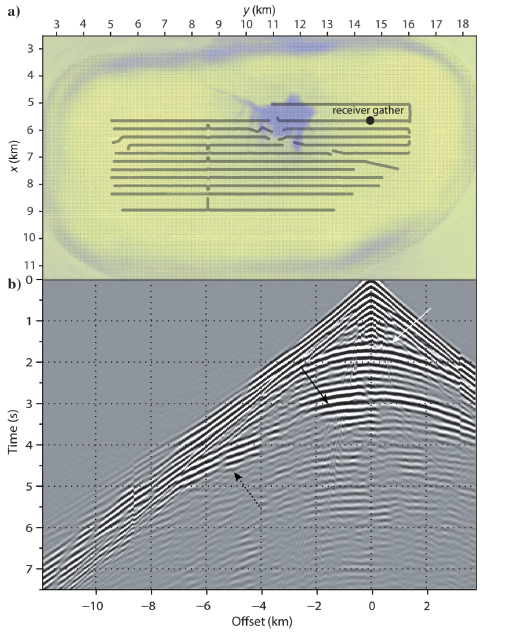
\includegraphics[width=0.6\textwidth]{images/sim1.png}
\caption{Full Wave Inversion (FWI) procedure. from []}
\label{sim1} 
% if you move the label it breaks the reference numbering; 
% always have it *after* the caption.
\end{figure}
The figure \ref{sim1}.a shows the gas cloud intersecting the cables (area covered by the 50,000 explosive sources) and the receiver position, whose records are shown in panel. In figure \ref{sim1}.b, the solid black arrow indicate precritical reflection from the reservoir, the dashed black arrow points to the critical and postcritical reflection, and the white arrow points to the reflection from the top of the gas [].

In the study of Operto et al., a case study of valhall data set shows approximately the presence of gas at 2.5km in depth []. With initial condition $V_0$, vertical-velocity, $\epsilon$ and $\delta$,  Thomsen's parameters, and the density $\rho = -0.0261 V^{2}_{0} + 0.373 V_0 + 1.458$ are used to apply frequency-domain FWI on the OBC data set []. With discrete frequencies chosen in the 3.5-10 Hz frequency band, the DSFDM/FWI code was performed in computer nodes that are equipped with two 2.5 GHz Intel Xeon IvyBridge E5-2670v2 processors with 10 cores per processor. the shared memory per node is 64 GB. The connecting network is InfiniBand fourth data rate (FDR) at 56 Gb/s. The operations are performed in single-precision complex arithmetic, for which the peak performance of the machine is 10 Gflops/s/core (which corresponds to a double precision peak of 20 Gflops/s/core). Figures \ref{sim2} \ref{sim3} show the 2D and 3D visualisations in different levels of the reservoir of the gas cloud.
According to the authors, this study reveals memory consumption in the step of LU factorisation. They showed that the complexity can reach $O (n^{6}) $ [].
%\begin{figure}[!h]
%% Use "\centering" in floats (figure, table), but if you need to center
%% some text (why?) use "\begin{center}...\end{center}".
%\centering 
%\begin{minipage}{0.6\textwidth}
%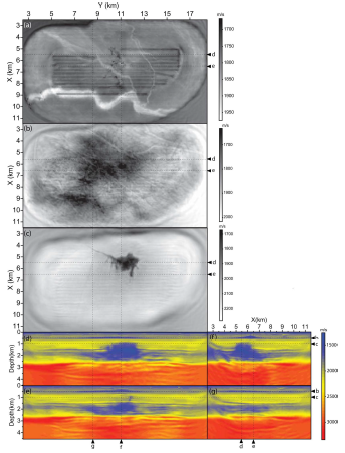
\includegraphics[width=0.6\textwidth]{images/sim2.png}
%\label{sim2} 
%\end{minipage}
%\hfill
%\begin{minipage}{0.6\textwidth}
%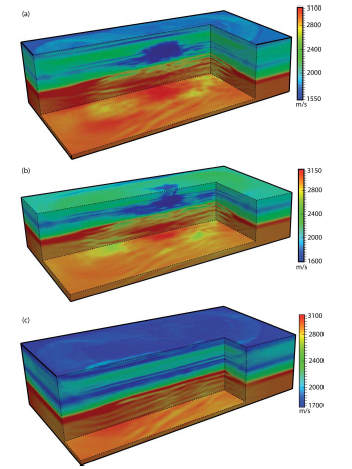
\includegraphics[width=0.6\textwidth]{images/3Dsim3.png}
%
%\label{sim3} 
%\end{minipage}
%\caption{Full Wave Inversion (FWI) procedure. from []}
%\end{figure}

\begin{figure}
\centering 
  \begin{subfigure}[b]{0.4\textwidth}
    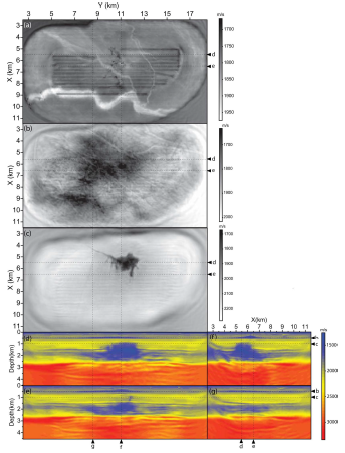
\includegraphics[width=\textwidth]{images/sim2.png}
    \caption{Picture 1}
    \label{sim2}
  \end{subfigure}
  %
  \begin{subfigure}[b]{0.4\textwidth}
    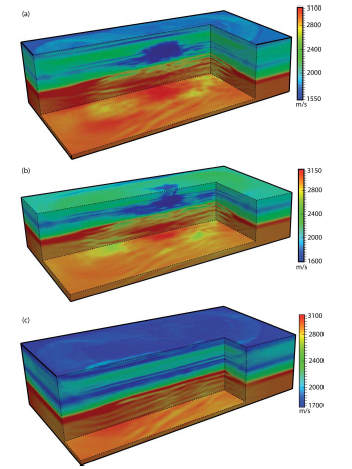
\includegraphics[width=\textwidth]{images/3Dsim3.png}
    \caption{Picture 2}
    \label{sim3}
  \end{subfigure}
\end{figure}
\section{High Performance Computing (HPC)} 
\subsection{Introduction to HPC}
Supercomputing has developed early in the 1970s with CDC 6600, ILLIAC-IV and the generation of CRAY. The high performance computing (HPC) was born in context of scientific computing. In fact, It was a challenge to be fast and more precise when were talking about scientific computing such as simulation purposes like weather forecasting, numerical mechanics for car crash tests, financial market prediction or other various complex phenomena modelings. The HCP's development was also accompanied with new paradigm in the computer design in hardware and software levels. It takes more advantages in the concepts of parallel system and parallel program, shared and distributed memory. Thus, the high performance computers as
machines with a good balance among the following major elements []:
\begin{itemize}
\item Multistaged (pipelined) functional units.
\item Multiple central processing units (CPUs) (parallel machines).
\item Multiple cores. 
\item Fast central registers.
\item Very large, fast memories.
\item Very fast communication among functional units.
\item Vector, video, or array processors.
\item Software that integrates the above effectively.
\end{itemize}

Today, with Moore's Laws, the performance of computer is continuously increasing. In 2017, the Top500\footnote{https://www.top500.org}, website ranking the list of the top 500 supercomputers, classifies the Sunway TaihuLight (a system developed by \textit{China's National Research Center of Parallel Computer Engineering \& Technology} (NRCPC)) to be the most power computer in the world. The Sunway TaihuLight has a note of 93 Petaflops in Linpack Performance, where a Petaflops is $10^{15}$ floating-point operations per second. Recently, the Atos group has launched a new generation of quantum learning machines that can reach 24 TB of memory and 16 CPU, with power of from 30 to 40 Qubits (see \ref{qlm}). These computers allows researchers, engineers and students to develop and experiment with quantum software.   
\begin{figure}[!h]
% Use "\centering" in floats (figure, table), but if you need to center
% some text (why?) use "\begin{center}...\end{center}".
\centering 
% Figure environments same as 0.8 * \textwidth please
% That does not necessarily mean the actual picture size,
% it is a guideline for the environment which could contain
% 2 or more pictures! Be consistent and follow the guidelines
% provided in your sources.
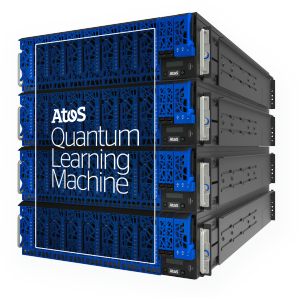
\includegraphics[width=0.4\textwidth]{images/qlm.png}
\caption{ATOS quantum learning machine}
\label{qlm} 
% if you move the label it breaks the reference numbering; 
% always have it *after* the caption.
\end{figure}
\subsection{HPC architecture}
Several effort has been doing in single processor performance by the ever-increasing density of transistors-the electronic switches-on integrated. The small dimension of transistors in an integrated circuit has increased the speed of this circuit. Therefore, this fact implies the increase of the heat of these transistors due to the power consumption. However, the air-cooled integrated circuits are reaching the limits of their ability to dissipate heat, in the first decade of the twenty-first century[]. 
Therefore, it is not sure to continue to increase the speed of integrated circuits. The chip's industries have another option instead to spend much money for building ever-faster, more complex, monolithic
processors. They decide to put multiple, relatively simple, complete processors on a single chip, called multicore[]. Each core represents a CPU. Now, Programmers have to take into account the parallel architecture to be more efficient and more faster. 
In the parallel systems, different concepts are used  : SIMD (\textit{Single Instruction, Multiple Data}), MIMD (\textit{Multiple Instruction, Multiple Data}), Shared Memory, Distributed Memory, Interconnection networks 
\begin{itemize}
\item \textbf{SIMD}: A concept of Flynn's taxonomy, SIMD indicates the fact that multiple processing units (core) execute the same instruction on multiple data streams. Each processing unit can perform on different data elements. The figure \ref{simb} gives an example of SIMD execution on three CPU.The SIMD is used for specialized problems characterized by a high degree of regularity, such as graphics/image processing (GPUs). In addition, SIMD is used in the architecture of vector processors which enable to vectorize loop in matrix calculation (see figure \ref{vector}).  
Example of SIMD Processor Arrays and Vector Pipelines : Thinking Machines CM-2, MasPar MP-1 \& MP-2, ILLIAC IV, IBM 9000, Cray X-MP, Y-MP \& C90, Fujitsu VP, NEC SX-2, Hitachi S820, ETA10.
\begin{figure}{!h}
\centering 
  \begin{subfigure}[b]{0.4\textwidth}
    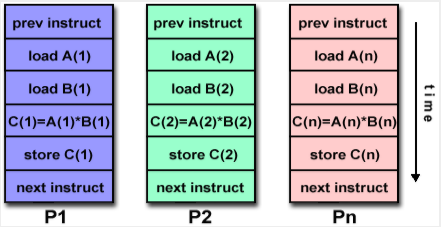
\includegraphics[width=\textwidth]{images/simd.png}
    \caption{Picture 1}
    \label{simb}
  \end{subfigure}
  %
  \begin{subfigure}[b]{0.4\textwidth}
    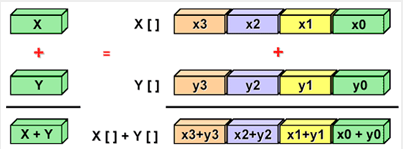
\includegraphics[width=\textwidth]{images/vectorization.png}
    \caption{Picture 2}
    \label{vector}
  \end{subfigure}
\end{figure}

\item \textbf{MIMD} As the name suggests, MIMD or multiple instruction streams on multiple processors (cores) operate on different data items concurrently. MIMD systems typically consist of a collection of fully independent processing units or cores, each of which has its own control and logical unit []. The execution process can be synchronous or asynchronous, deterministic or non-deterministic []. The MIMD architecture is found in most current supercomputers, networked parallel computer clusters and "grids", multi-processor SMP computers, multi-core PCs. The figure  shows an example of MIMD execution.  
\begin{figure}[!h]
\centering 
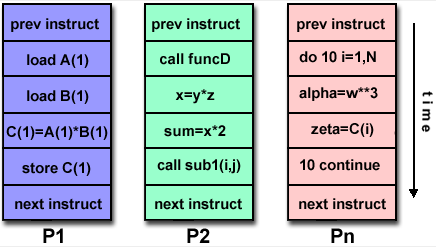
\includegraphics[width=0.6\textwidth]{images/mimd.png}
\caption{Picture []}
\label{sim1} 
% if you move the label it breaks the reference numbering; 
% always have it *after* the caption.
\end{figure}

\item \textbf{Shared Memory} A shared-memory system is a collection of autonomous processors (cores) connected to memory via an interconnection network, and processors share physical address of memory \cite{}. There are two different memory access in shared-memory system: Uniform Memory Access (UMA) and cache-coherent Non-uniform Memory Access (ccNUMA). 

The UMA can be considered a 'flat' memory model, because latency and an bandwith are the same for all cpu and all memory location. Sometimes called Symmetric Multiprocessor (SMP), UMA system  enables to have equal access and equal time to memory. The general problem of UMA machines is that bandwidth bottlenecks are bound to occur when the number of sockets is larger than a certain limit \cite{}. The figure \ref{uma} show a representation of UMA architecture. 
In ccNUMA, memory is physically distributed but logically shared (see figure \ref{numa}). This architecture seems to be distrubuted-memory system, but network logic makes the aggregated memory of the whole system appear as
one single address space \cite{}. This simplify the memory access without resorting to a network of any kind. The locality domain (LD), set of processor cores connected locally to memory,can be considered as a UMA "building block". The ccNUMA principle gives scalable bandwidth for very large processor counts. It can be inexpensive small for two- or four-socket nodes frequently used for HPC clustering \cite{}.

The LD can be, sometimes, an obstacle for high performance software on ccNUMA. The second problem is potential
contention if two processors from different locality domains access memory in the same locality domain, fighting for memory bandwidth. Both problems can be solved by carefully observing the data access patterns of an application and restricting data access of each processor to its own locality domain \cite{}.
\begin{figure}[!h]
\centering 
  \begin{subfigure}[b]{0.4\textwidth}
    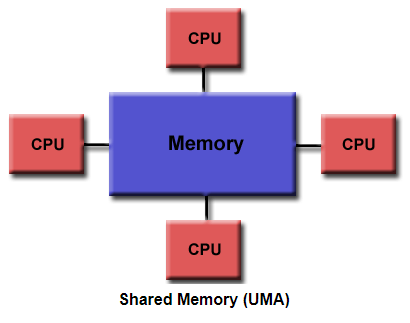
\includegraphics[width=\textwidth]{images/uma.png}
    \caption{}
    \label{uma}
  \end{subfigure}
  %
  \begin{subfigure}[b]{0.4\textwidth}
    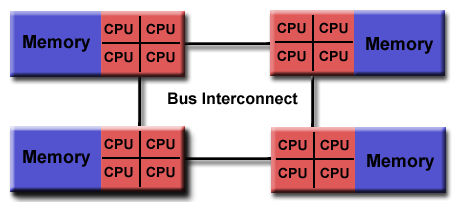
\includegraphics[width=\textwidth]{images/numa.png}
    \caption{}
    \label{numa}
  \end{subfigure}
\end{figure}
\item \textbf{Distributed Memory}
In the distributed-memory system, each processor is connected to exclusive local memory and network communication connect also inter-processor memory (see \ref{dmemory}). The memory is scalable with the number of processor and we are a rapid access of each processor with its own memory. However, the programmer must explicitly define how to access data when a processor need it in another one. Besides, the programmer is also responsible to handle the synchronization task \cite{}.
\begin{figure}[!h]
\centering 
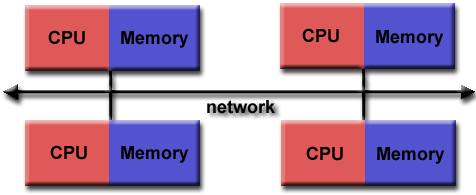
\includegraphics[width=0.4\textwidth]{images/d-memory.png}
\caption{Distributed Memory}
\label{dmemory} 
\end{figure}

According to \cite{}, there are actually no distributed-memory systems any more that implement such a layout where we HPC clustering. Most of parallel systems couple at same time shared and distributed systems (Hybrid Systems) i.e. there are shared-memory building blocks connected via a fast network. This Hybrid Distributed-Shared Memory make the system to take advantages of the two architectures and the increase of the scalability. The figure \ref{hybrid} shows an Hybrid architecture with CPU and GPU (\textit{Graphical Processing Unit}) cores.
\begin{figure}[!h]
\centering 
  \begin{subfigure}[b]{0.4\textwidth}
    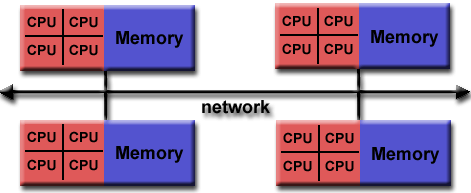
\includegraphics[width=\textwidth]{images/hybrid1.png}
  \end{subfigure}
  %
  \begin{subfigure}[b]{0.4\textwidth}
    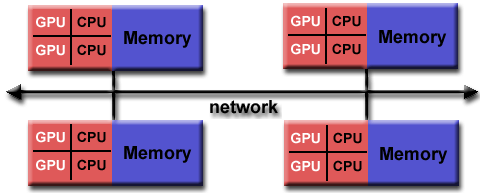
\includegraphics[width=\textwidth]{images/hybrid2.png}   
  \end{subfigure}
   \label{hybrid}
   \caption{Hybrid System with CPU/GPU cores}
\end{figure}
\item \textbf{Interconnection networks}
In HPC domain, the interconnect plays a crucial role for latency and bandwidth performance of both distributed- and shared-memory systems.

\begin{figure}[!h]
\centering 
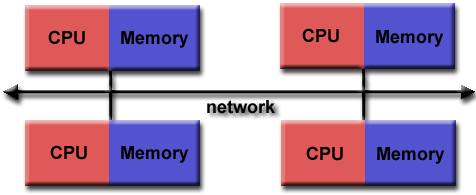
\includegraphics[width=0.4\textwidth]{images/d-memory.png}
\caption{Interconnected Networks with different topologies}
\label{dmemory} 
\end{figure}
\end{itemize}

\subsection{Parallel Programming} \label{scalability}

\begin{itemize}
\item \textbf{Speedup}
\item \textbf{Amdhal's Law}
\item \textbf{Gustafson's Law}
\item \textbf{Scalability}
\end{itemize}

\subsection{Shared Memory Parallel Programming: OpenMP} \label{openMP}
\subsection{Distributed Memory Parallel Programming: MPI}
\subsection{Challenges of HPC in the context of 3D Seismic Imaging}



 % Chapters might go from 2. problem statement, 
                 % through 3. model, to 4. analysis & results
\chapter{Optimization Techniques in a Parallel System} \label{optimization}

\section{Compiler Optimization}
\section{Threading/Multi-threading}
\section{Vectorization}
\section{Placement of MPI processes}
\section{Code Profiling}
\section{Optimization Libraries}
\section{Hardware Accelerators}




 % You do not need to have exactly 4 chapters.
                 % It is probably a good minimum, with 5 chapters 
                 % average, and 7 chapters might be a maximum.
\chapter{Optimization of DSFDM/FFWI code in shared node, MESCA II}
\section{DSFDM/FFWI}
\subsection{Description}
The DSFDM/FFWI is a package which contains parallel computer codes to perform seismic modeling and fullwaveform inversion in the frequency domain. These codes have have been designed to execute modeling/inversion in 1, 2, 3 dimension media. According to the authors, only the 3D version is tested and Documented [doc DSfDm]. The DSFDM code is the seismic modeling code, while the FFWI code performs the inversion, using most of the subroutines implemented in DSFDM.Moreover,the DSFDM/FFWI codes assume visco-acoustic submarine supports in which vertical transverse isotropy can be taken into account.

Seismic modeling is performed in the frequency domain with a finite-difference method on a uniform Cartesian grid ([Operto et al., 2007][Brossier et al., 2010]; [Operto et al., 2014]). The linear system resulting from
the discretization of the time-harmonic wave equation is solved with a sparse direct solver. Sources and receivers, which can be processed in a reciprocal way, can be considered at arbitrary positions in coarse finite-difference grids with the sinc parameterization developed by Hicks (Hicks, 2002). Absorbing boundary conditions are perfectly-matched layers (PMLs) ([B\'{e}renger, 1994]; [Operto et al., 2007]). A free-surface boundary condition can be used along arbitrary tomography by forcing the pressure wave-field to 0 along this boundary. All of the tasks performed during seismic modeling (building impedance matrix, building right-hand side vectors, call of MUMPS subroutines, writing of solutions and extraction at receiver solutions) are implemented in the DSFDM code.

FFWI code is implemented with various local optimization methods. Recorded data are provided in the frequency-domain using an adaptation of the Seismic Unix (SU) format. The data are complex-valued (in single precision) and the frequency interval is uniform. The first frequency, the number of frequency and the frequency interval must be provided at specific locations in the SU headers. The numerical optimization is performed with the SEISCOPE optimization toolbox and allows for steepest-descent, conjugate gradient,l-BFGS and truncated Newton optimizations ([M\'{e}tivier and Brossier, 2016]). Seismic modeling and inversion are performed on the same Cartesian grid. Source wavelet estimation can be performed at each iteration of the FWI. Only the preconditioned steepest-descent optimization was tested, although conjugate gradient and l-BFGS optimizations are interfaced with the FFWI code. Interfacing Gauss-Newton and Newton truncated optimizations is the aim of ongoing work. The code has been tested for the update of the vertical wavespeed only. An application to real data is shown in [Operto et al., 2015]. Multi-parameter gradients are implemented but still need to be validated.

\section{MUMPS Solver}
MUMPS ("MUltifrontal Massively Parallel Solver") is a package for solving systems of linear equations of the form $ Ax = b$, where $ A $ is a square sparse matrix that can be either unsymmetric, symmetric positive definite, or general symmetric, on distributed memory computers. The MUMPS package is designed to solve linear equations by using a direct method based on a multifrontal approach which performs a Gaussian factorization
$$ A = LU $$ 
where $ L $ is a lower triangular matrix and $ U $ an upper triangular matrix. If the matrix is symmetric then
the factorization
$$ A = LDL^{T}$$
where D is block diagonal matrix with blocks of order 1 or 2 on the diagonal is performed. 

MUMPS solvers the result of collaboration between different partners working in the MUMPS project since 1996. Todays, the MUMPS team include CERFACS, CNRS, ENS-Lyon, INRIA, INPT, University of Bordeaux. In the recent years, the popularity of MUMPS package has increased in different countries and different scientific projects. It has known different version during the years with real improvement of the LU factorization methods. The recent research of MUMPS project is focused on the Block-Low rank option that allows decreasing the complexity of sparse direct solvers on problems arising from partial differential equations is provided for experimentation purpose. 

A matrix A of size $ m \times n $ is said to be low rank if it can be approximated by a low-rank product $ \tilde{A} = XY^{T}$ of rank $ k_{\epsilon} $, such that $ k_{\epsilon}(m+n)\leq mn $ and $ \Vert \tilde{A} - A \Vert \leq  k_{\epsilon} $. The first condition states that the low-rank form of the matrix requires less storage than the standard form, whereas the second condition simply states that the approximation is of good enough accuracy. Using the low-rank form also allows for a reduction of the number of floating-point operations performed in many kernels (e.g., matrix-matrix multiplication).

Thanks to the low-rank compression, the theoretical complexity of the factorization is reduced from $ O(n^{6})$ to $ O(n^{5.5})$ and can be further reduced to $ O(n^{5} \log 5 )$ with the best variant of the BLR format ([Amestoy et al., 2016b]).

\section{Tools}
As we mentioned above, this DSFDM/FFWI version use MUMPS package to solve the linear system of discretized wave propagation equation. We need to install different packages for MUMPS dependencies as well as DSFDM/FFWI. MUMPS can be installed in sequential version. In the same way, it can be used with multithreaded machine (with OpenMP) or with parallel version (distributed memory MPI based). We need these packages for MUMPS installation:
\begin{itemize}
\item \textbf{BLAS library}: BLAS (\textit{Basic Linear Algebra Subprograms}) are routines that provide standard building blocks for performing basic vector and matrix operations. The Level 1 BLAS perform scalar, vector and vector-vector operations, the Level 2 BLAS perform matrix-vector operations, and the Level 3 BLAS perform matrix-matrix operations. BLAS is written in Fortan and it has an optimized sequential or multithreaded version.
\item LAPACK library: LAPACK or Linear Algebra PACKage routines are written so that as much as possible of the computation is performed by calls to the Basic Linear Algebra Subprograms (BLAS). LAPACK is designed at the outset to exploit the Level 3 BLAS. Because of the coarse granularity of the Level 3 BLAS operations, their use promotes high efficiency on many high-performance computers, particularly if specially coded implementations are provided by the manufacturer.
\item ScaLAPACK library: Similar to LAPACK, ScaLAPACK is a library of high-performance linear algebra routines for parallel distributed memory machines. It solves dense and banded linear systems, least squares problems, eigenvalue problems, and singular value problems. The use of ScaLAPACK provides efficiency, scalability, reliability, portability, flexibility, and ease of use (by making the interface to LAPACK and ScaLAPACK look as similar as possible). 
\item BLACS library: In the context of distributed parallel machines, the BLACS (Basic Linear Algebra Communication Subprograms) routines is created to make easy linear algebra oriented message passing interface that may be implemented efficiently and uniformly across a large range of distributed memory platforms.
\item OpenMP library: As we discuss in the section \ref{openMP}, this package allows parallel programming in  shared memory multi-core platforms. The openMP directives improves strongly the performance of MUMPS. OpenMP parallel regions of MUMPS can be set through the OMP\_NUM\_THREADS environment variable. 
\item MPI library: 
\item Others
\end{itemize}

\section{Installation of DSFDM/FFWI}
\subsection{Description of nodes}
\section{Methodology}
In this study, our aim is to evaluate the capacity of the DSFDM/FFWI code to process large test cases on MESCA-II node and to improve the performance of the code in this architecture. This implies how to keep the code scalable when the memory consumption and MPI communications are increasing. In [], the authors show that the memory consumption and elapsed time are mostly based on LU matrix factorisation doing by MUMPS package. Their results explain in more details this fact [].  The MUMPS team has developed the BLR option to improve the performance of the storing of LU matrix values (Amestoy et al. []). 
As we discuss above (see \ref{optimization}), the optimization of DSFDM/FFWI can be seen in multiple levels. In this study, we will focus on scalability study (strongly and weakly) and different profiling methods to analyse the performance of the code.  
\section{Scalability study}
The scalability, as we discussed in section \ref{scalability}, is the coarse grained of the study of performance. It can be measured in two scales: strong scaling and weak scaling. Here, we study these two scales in different  nodes cluster such as Mesca and classical nodes. When we say classical nodes it refers the other nodes different to Mesca.  
\subsection{Strong Scalability}
This study allow us to understand how much faster our DSFDM/FFWI code is with N processors by fixing the size of the problem. Firstly, we perform different test cases in classical nodes to be comparing the performance with Mesca. To study the scalability, we use the homogeneous isotropic model that aims to validate DFSFDM against an analytical solution computed in an homogeneous infinite acoustic isotropic ($ianiso=0$) medium (Docffwi). According to the documentation, we fix, firstly, the size of the problem to be grid $(n1,n2,n3)=(41,41,121)$ ie. $ 4km \times 4km \times 12km$ (depth,X,Y). The others parameters are the same as the documentation. The wavespeed and the density are respectively equal to $ 1.5km/s $ and $ 1000km/m3 $. The grid interval is $ 100m$. The frequency is $3.72Hz$. The shot coordinates in meters are $ (x1, x2, x3) = (1000, 2000, 2000)$.

The results obtained in Figures \ref{cube_homogeneous_isotropic}-\ref{fig2_log_homogeneous_isotropic} show the comparison of \textbf{DSFDM} with the analytical solution (\textbf{FDTD}).
 
In the first test case, we run the code in a classical node such that the architecture is given in Table \ref{mannyNode} \newline

\begin{table}[!h]
\centering

\begin{tabular}{|l|l|}
\hline
Number of sockets (CPUs) & 2 sockets Intel(R) Xeon(R) CPU E5-2697 v2 	\\	
\hline
Number of Core(s) & 2 * 12 cores per socket at the nominal frequency 2.70GHz	\\	
\hline
Hyperthreading & activated			\\
\hline
Number of Thread(s) &  2 * 24 threads per cpu	\\
\hline
Shared Memory & 2*32 GB DDR*  (* unknown) \\	
\hline		
L1d/L1i cache &         32K	\\		
\hline
L2 cache &              256K	\\	
\hline	
L3 cache &             30720 KB	\\
\hline
\end{tabular}
\caption{Architecture of classical nodes}
\label{mannyNode}
\end{table}

The table \ref{manny} shows the computational resources used when the code is performing in this node.
\begin{table}[!h]
\centering

\begin{tabular}{lllllllll}
Grid dimensions & npml & \#u & \#n & \#MPI & \#th & $Mem_{LU}(Gb)$ & $T_{LU}(s)$ & $T(s)$ \\
 \hline
$41 \times 41 \times 121$ & 8 & 1 & 1 & 2  & 10 & 6,7 &  17.76 & 23.77 
\end{tabular}
\caption{Homogeneous Isotropic running on classical node: \#u($ 10^{6} $): number of unknowns. \#n: number of nodes. \#MPI: number of MPI process. \#th: number of threads per MPI process. $Mem_{LU}(Gb)$: Memory for LU
factorization in Gbytes. $T_{LU}(s)$: Elapsed time for factorization in s. $ T(s)$: Running time}
\label{manny}
\end{table}

Secondly, we execute the same test case with the same parameters in the Mesca node. The architecture of this node is showing in table \ref{mescaNode}.

\begin{table}[!h]
\centering
\begin{tabular}{|l|l|}
\hline
Number of sockets (CPUs) & 8 sockets Intel(R) Xeon(R) CPU E7-8890 v4 	\\	
\hline
Number of Core(s) & 8 * 24 cores cores at the nominal frequency 2.20GHz	\\	
\hline
Hyperthreading & deactivated			\\
\hline
Number of Thread(s) &  8 * 24 threads per cpu	\\
\hline
Shared Memory & 8*340 GB DDR*  (* unknown)   \\	
\hline		
L1d/L1i cache &         32K	\\		
\hline
L2 cache &              256K	\\	
\hline	
L3 cache &              61440K	\\
\hline
\end{tabular}
\caption{Architecture of Mesca II node}
\label{mescaNode}
\end{table}

These results are shown in the table \ref{Mesca1}

\begin{table}[!h]
\centering

\begin{tabular}{lllllllll}
Grid dimensions & npml & \#u & \#n & \#MPI & \#th & $Mem_{LU}(Gb)$ & $T_{LU}(s)$ & $T(s)$ \\
 \hline
$41 \times 41 \times 121$ & 8 & 1 & 1 & 2  & 10 & 6,7 &  17.73 & 25.048 
\end{tabular}
\caption{Homogeneous Isotropic running on Mesca II node}
\label{Mesca1}
\end{table}

By using two MPI processes and ten threads, the classical node shows almost the same performance as Mesca(
 $T_{LU}(s)\thickapprox 17.7 s$). In addition, the total memory allocated for factorization was  6.7 Gigabyte.The time of LU factorization takes 74 \% and 70 \% respectively in the classical node and Mesca. This type of node will be used for rest of the simulation. The results are shown in tables \ref{Mesca1} and \ref{manny}. \newline
\begin{figure}
\centering 
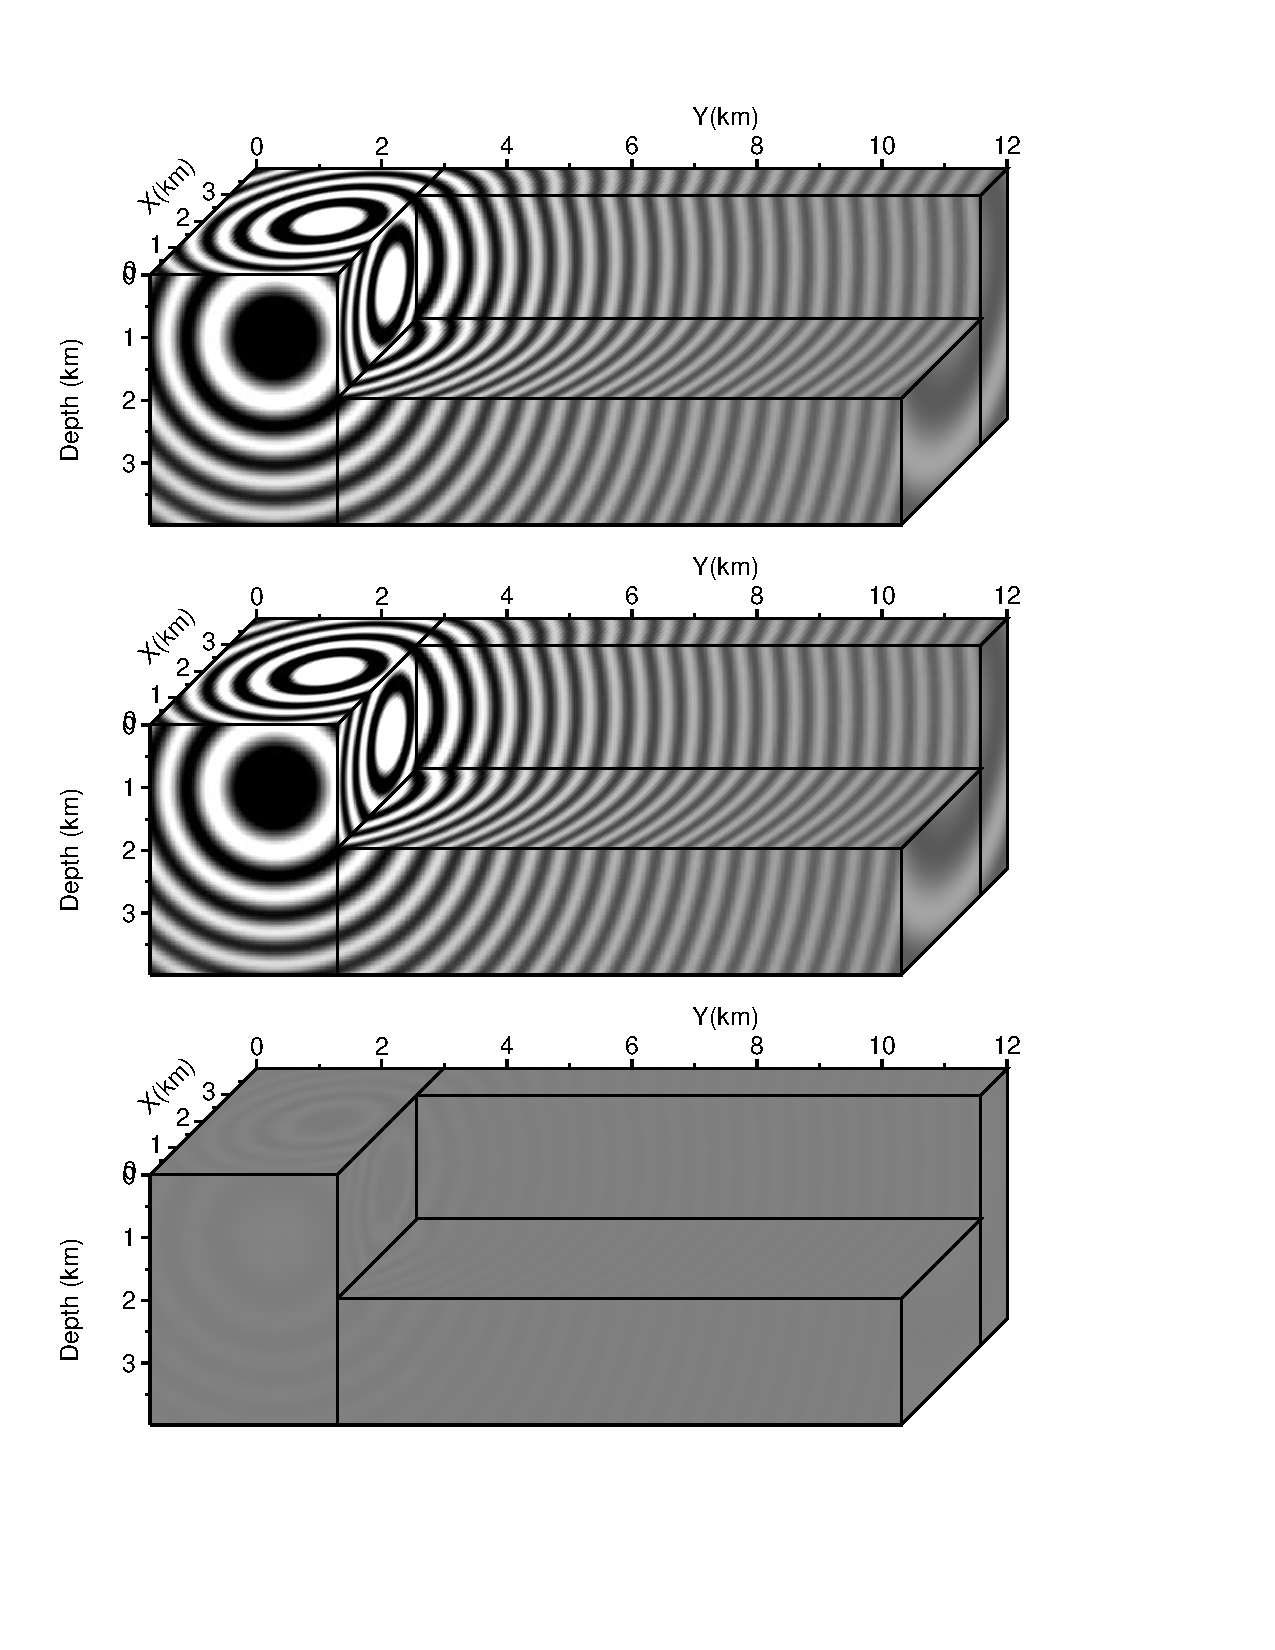
\includegraphics[width=0.7\textwidth]{images/fig_dsfdm/fig_cube_homogeneous_isotropic.pdf}
\caption{Homogeneous Isotropic. Infinite homogeneous isotropic medium. Validation against analytical
solution. a) DSFDM solution. b) Analytical solution. c) Difference.}
\label{cube_homogeneous_isotropic} 

\end{figure}
\begin{figure}[]
\centering 
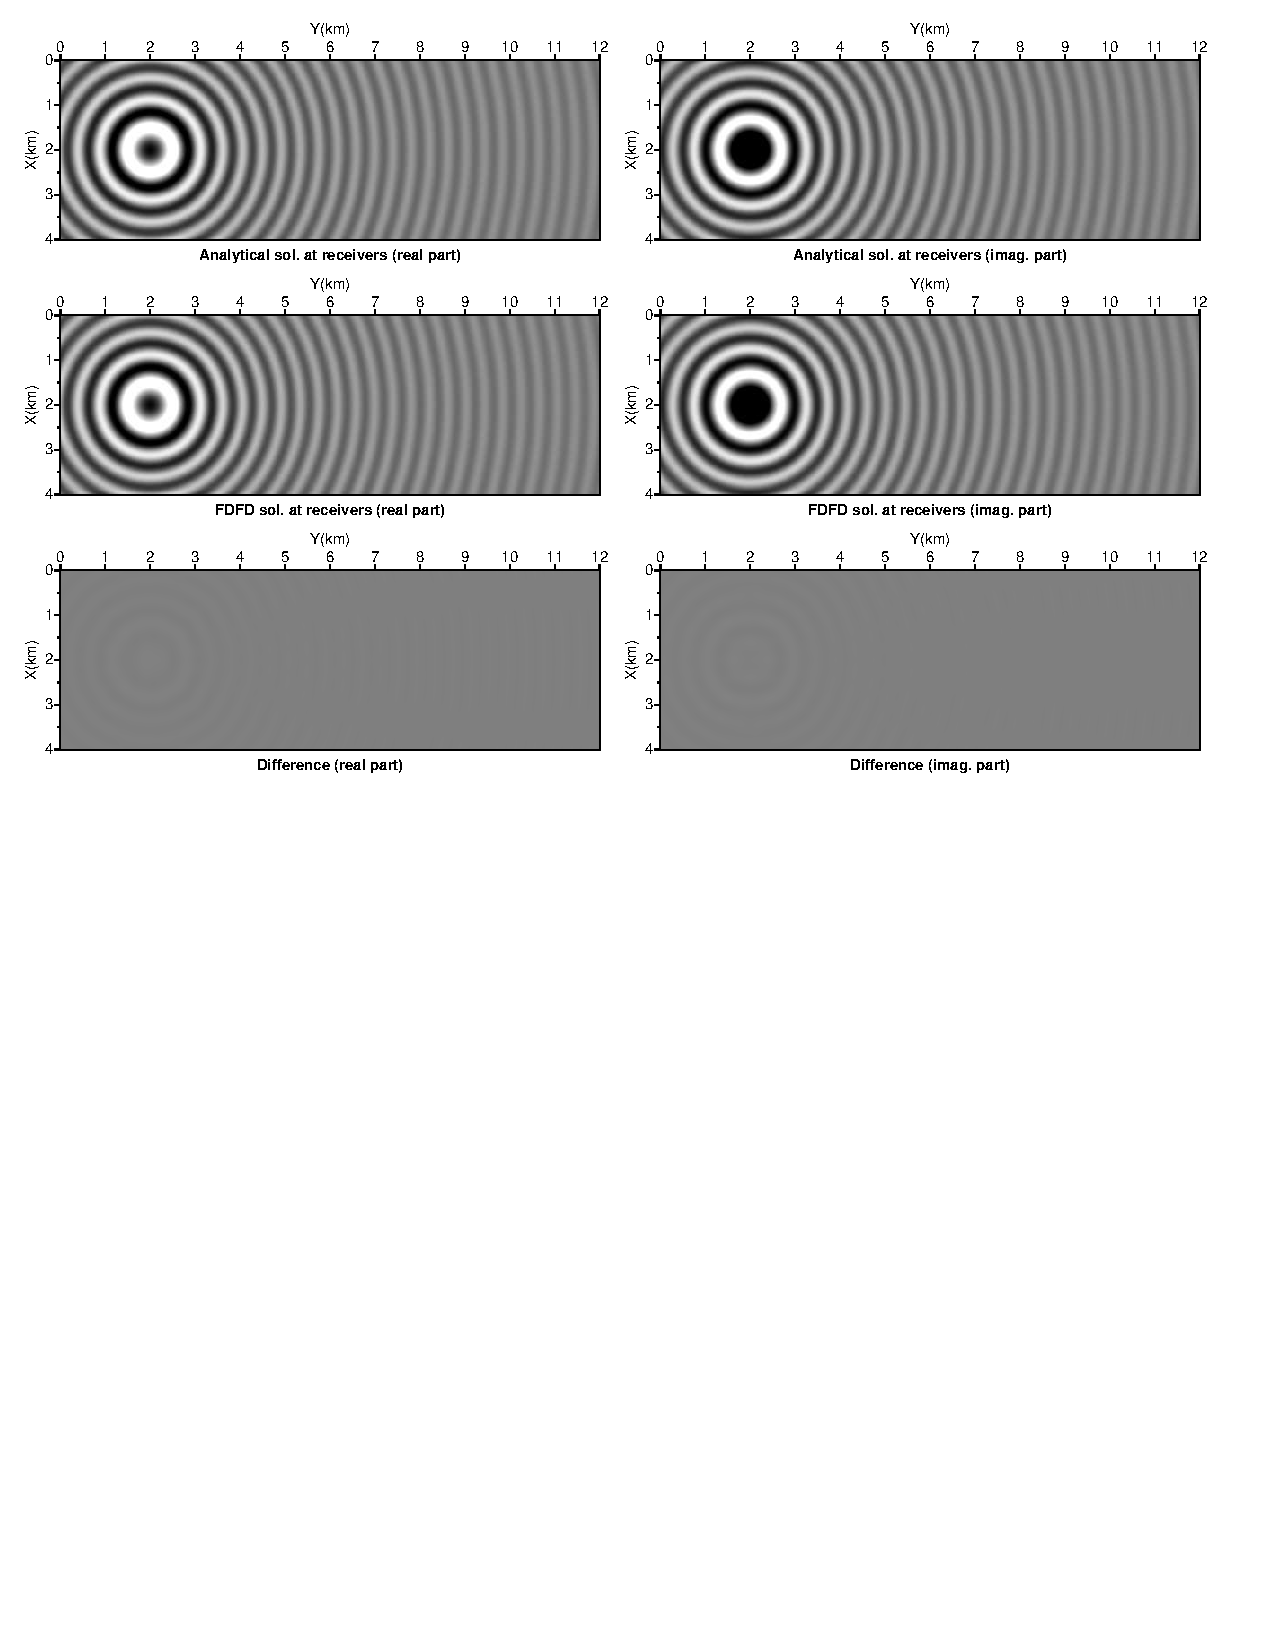
\includegraphics[width=0.7\textwidth]{images/fig_dsfdm/fig_rec_snap_homogeneous_isotropic.pdf}
\caption{Homogeneous Isotropic.  Infinite homogeneous isotropic medium. Validation against analytical
solution. Solution at receiver positions, 1km below the surface.}
\label{rec_snap_homogeneous_isotropic} 
\end{figure}
\begin{figure}[]
\centering 
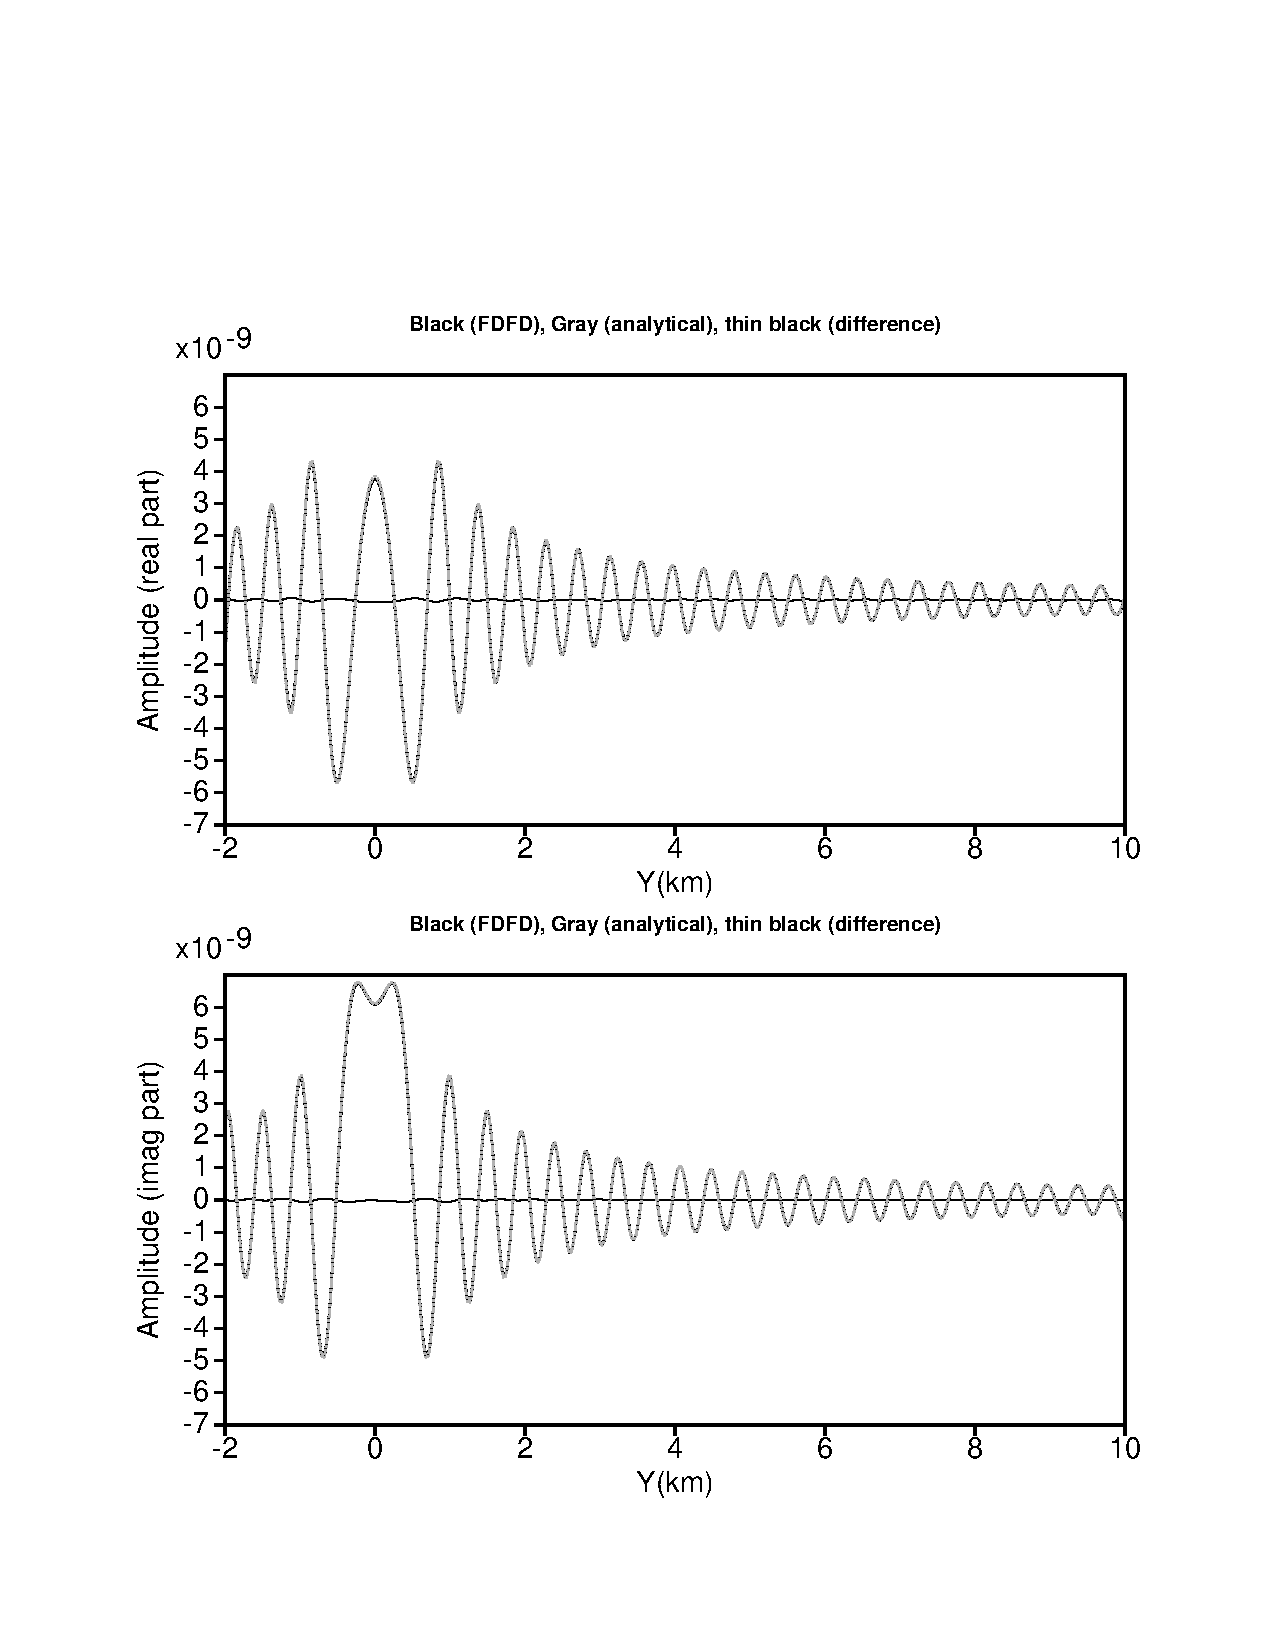
\includegraphics[width=0.7\textwidth]{images/fig_dsfdm/fig_rec_log_homogeneous_isotropic.pdf}
\caption{Homogeneous Isotropic. Infinite homogeneous isotropic medium. Validation against analytical
solution. Solution at receiver positions along the Y profile running across the shot position.}
\label{rec_log_homogeneous_isotropic} 
\end{figure}
\begin{figure}[]
\centering 
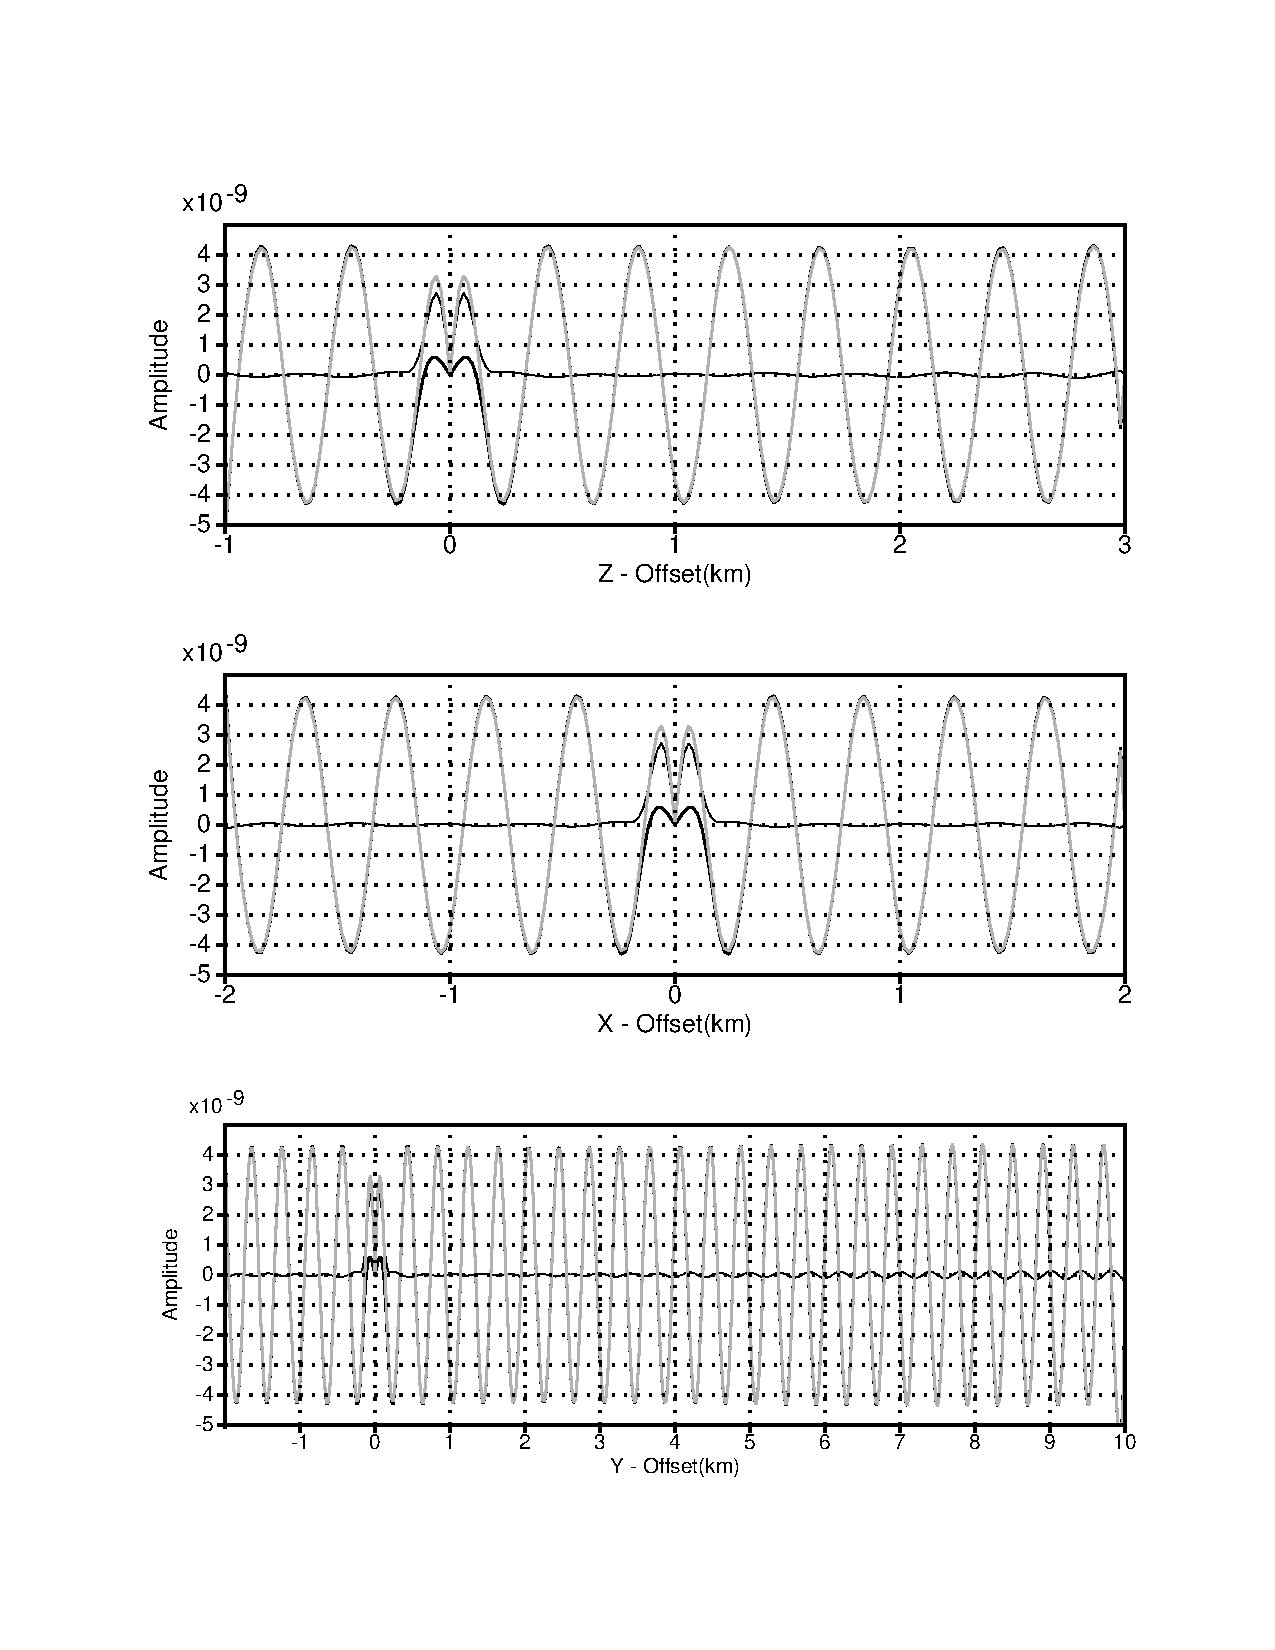
\includegraphics[width=0.7\textwidth]{images/fig_dsfdm/fig1_log_homogeneous_isotropic.pdf}
\caption{Homogeneous Isotropic. Infinite homogeneous isotropic medium. Validation against analytical
solution. Logs across shot position with correction for geometrical spreading}
\label{fig1_log_homogeneous_isotropic} 
\end{figure}
\begin{figure}[]
\centering 
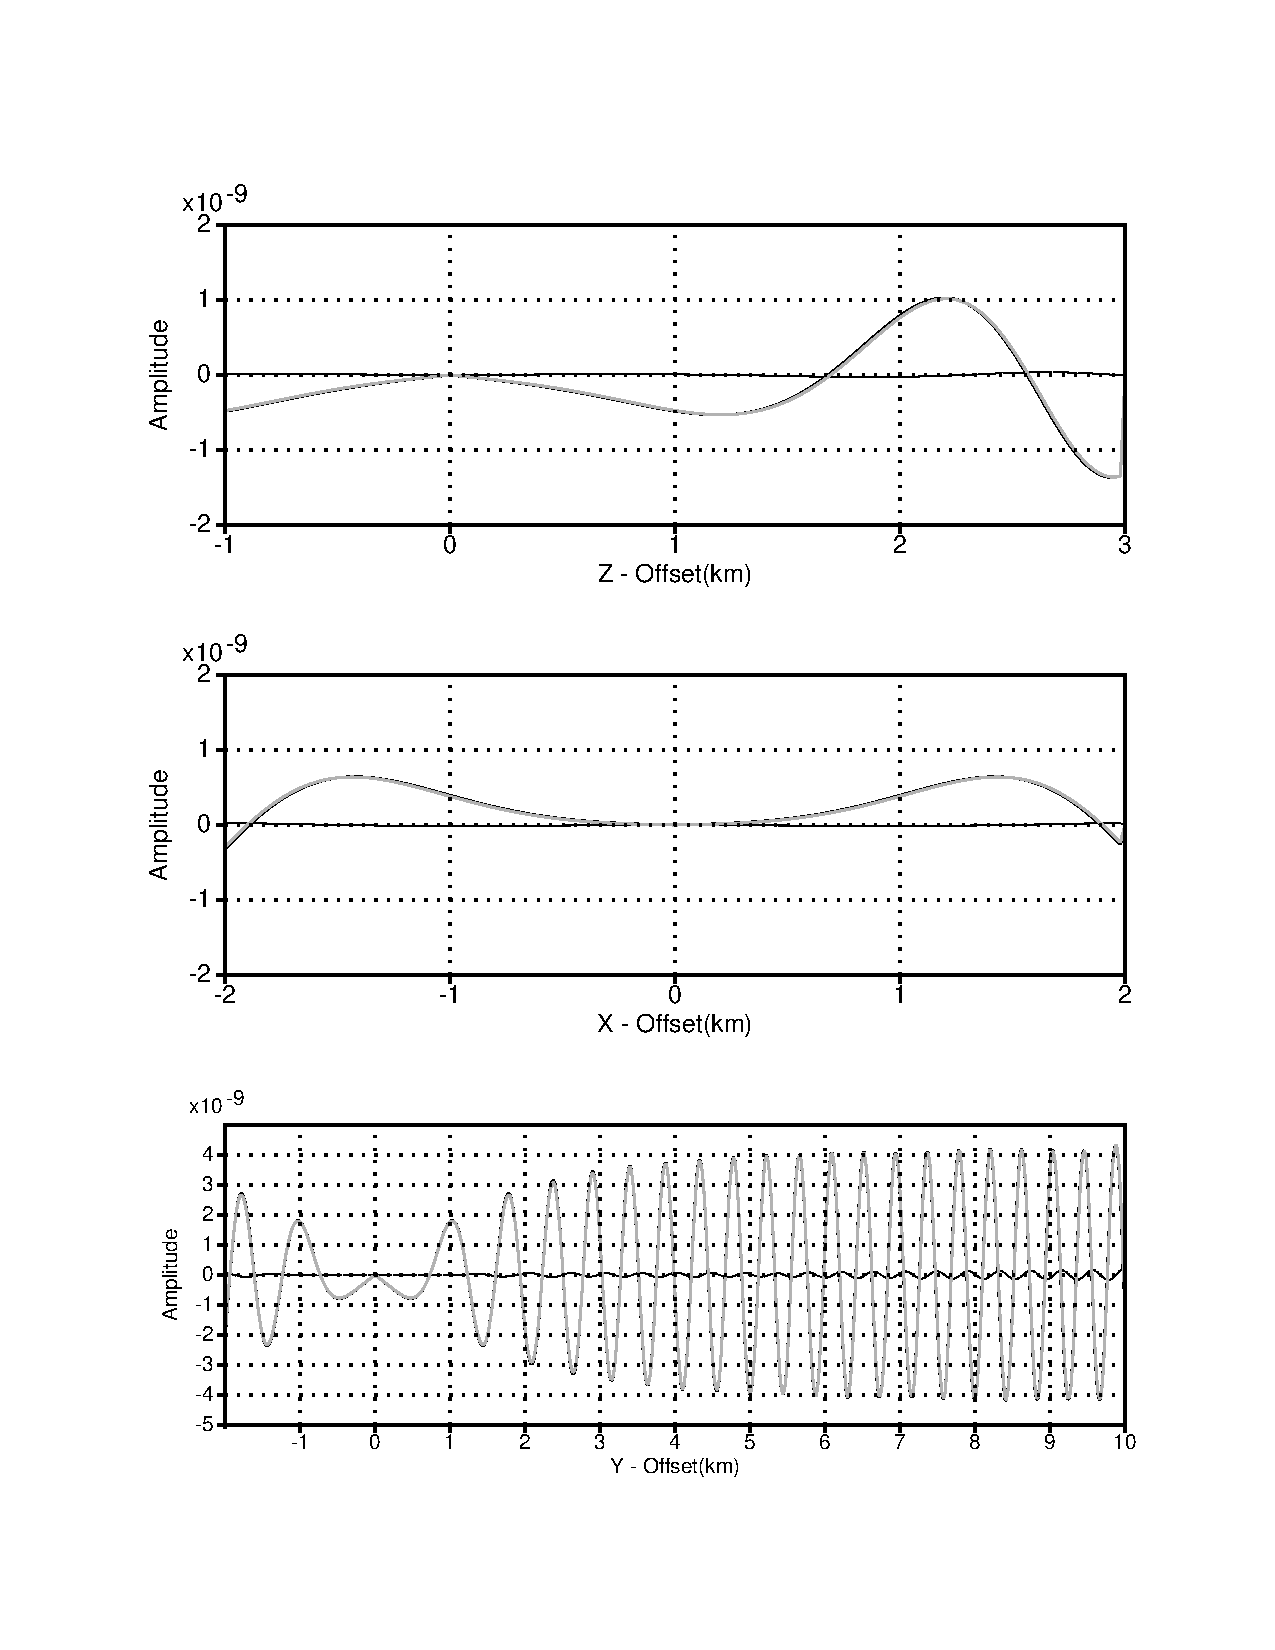
\includegraphics[width=0.7\textwidth]{images/fig_dsfdm/fig2_log_homogeneous_isotropic.pdf}
\caption{Homogeneous Isotropic. Infinite homogeneous isotropic medium. Validation against analytical
solution. Logs along the slices of Fig. ??b with correction for geometrical spreading}
\label{fig2_log_homogeneous_isotropic} 
\end{figure} 

In the following sentences, we define three test cases depending on the size of the grid to study the strong scalability of DSFDM code. This grid is a 3D dimension, $n1, n1, n1$, with PMLs. The chosen sizes of the grid are  $(n1,n2,n3)=(81,81,121)$,  $(n1,n2,n3)=(81,121,121)$ and $(n1,n2,n3)=(121,121,121)$. The grid interval is 100. We perform these tests in node cluster which contains the classical nodes and Mesca node described above. The resolution of wave propagation equation is handled by MUMPS solver. Here, we are more interested in factorization phase performing by MUMPS solver. This factorization can be doing in two ways: Full Rank and Low-Block Rank. In the following simulation, we will focus on the Full Rank option. In all the tests, we consider the number of MPI processes is always less or equal than the number of sockets (or CPU). 

The Figures \ref{TimeLU} and \ref{TimeMPIlog} show the elapsed time of the three different test cases running on classical nodes. As we can see in Figure \ref{TimeLU}, the Time of LU factorization depending on numbers of processes decreased by following a power law decay. We remark also, we obtain a good approximation when the numbers of processes is equals to a power of 2 (see Figure \ref{TimeLU2}). A log-log plot, (Figure \ref{TimeMPIlog1}), shows the strong scalability of the tests. In the case of $(n1,n2,n3)=(121,121,121)$, we observe a rapid drop of elapsed time between 2 and 8 processes and smooth descent of the curve in 8 and 16. The table \ref{fitting} shows the curve fitting of the the log scale plots (ie. $ Y= A*log(N)+B $, with N number of processes).

\begin{table}[!h]
\centering
\begin{tabular}{l|l|l}
Size & A & B  \\
 \hline
$81 \times 81 \times 121$ & -0.65 & 2.17	 \\
 $81 \times 121 \times 121$ & -0.71 & 2.5 \\
$ 121 \times 121 \times 121$ &  -0.75 & 2.86 

\end{tabular}
\caption{Parameters of the fitting curves of Elapsed time in classical nodes}
\label{fitting}
\end{table}

Similarly, we get the same remark in Mesca node (see Figure \ref{TimeMPIlog}). Here, we see a rapid growth between 2 and 4 processes different of the classical nodes. The elapsed time is fitted in log scale plot such that the slope and the intercept are given by the table \ref{fittingMesca}. For comparing the performance of Mesca and the classical nodes, we can use the execution time or the elapsed time in LU factorization. As the two architectures are different,   time may not be a good measure of comparison. We can can go further by considering the speedup that is define by Amdhal.

\begin{table}[!h]
\centering
\begin{tabular}{l|l|l}
Size & A & B  \\
 \hline
 $81 \times 81 \times 121$ & -0.62 & 2.16	\\
$81 \times 121 \times 121$ & -0.74 & 2.5 \\
$121 \times 121 \times 121$ &  -0.72 & 2.81

\end{tabular}
\caption{Parameters of the fitting curves of Elapsed time in Mesca}
\label{fittingMesca}
\end{table}



\begin{figure}
\centering 
  \begin{subfigure}[b]{0.7\textwidth}
    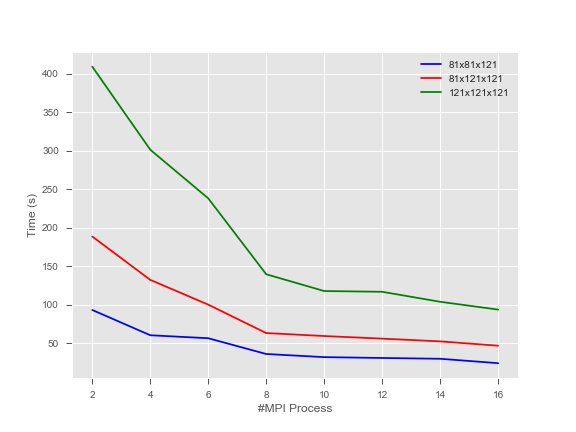
\includegraphics[width=\textwidth]{images/TimeLU.png}
    \caption{Time Elapsed for LU factorization performing in classical nodes}
    \label{TimeLU}
  \end{subfigure}
   
   \begin{subfigure}[b]{0.7\textwidth}
    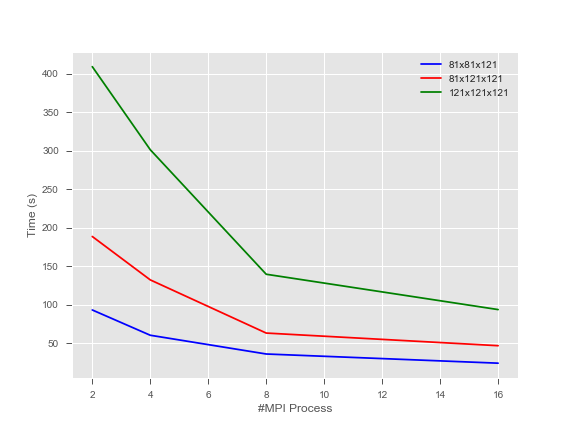
\includegraphics[width=\textwidth]{images/TimeLU2.png}
    \caption{Elapsed time for LU factorization in log scale performing in on classical nodes}
    \label{TimeLU2}
  \end{subfigure}
  
  %
  \begin{subfigure}[b]{0.7\textwidth}
    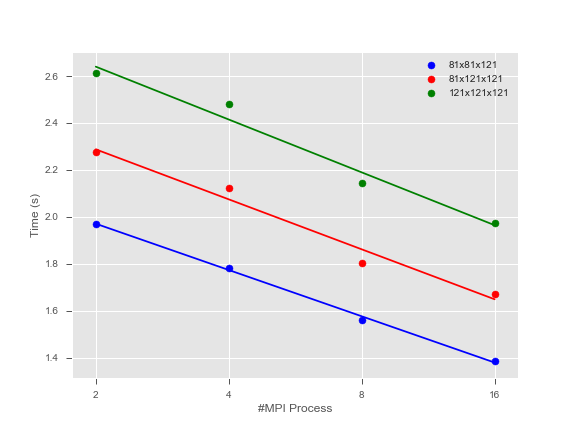
\includegraphics[width=\textwidth]{images/TimeMPIlog1.png}
    \caption{Elapsed time for LU factorization in log scale performing in on classical nodes}
    \label{TimeMPIlog}
  \end{subfigure}
  
\end{figure}
 
\begin{figure}
\centering 
  \begin{subfigure}[b]{0.7\textwidth}
    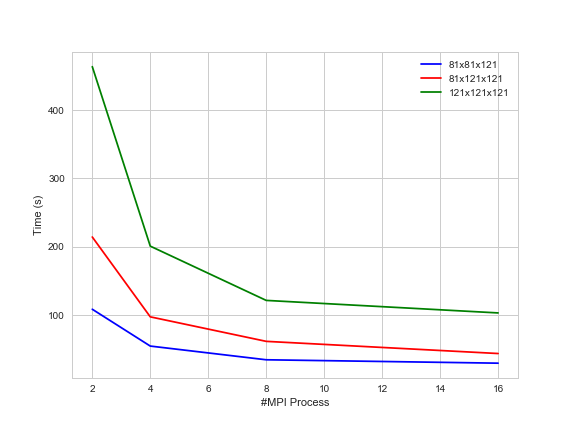
\includegraphics[width=\textwidth]{images/TimeMescaLU.png}
    \caption{Time Elapsed in LU factorization in  performing in Mesca node}
    \label{TimeMescaLU}
  \end{subfigure}
  %
  \begin{subfigure}[b]{0.7\textwidth}
    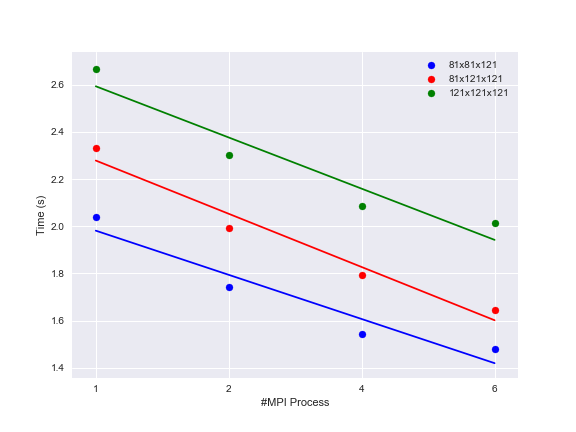
\includegraphics[width=\textwidth]{images/TimeMescaMPIlog.png}
    \caption{Elapsed time for LU factorization in log scale performing in Mesca node}
    \label{TimeMescaMPIlog}
  \end{subfigure}
\end{figure} 

\begin{figure}
\centering 
  \begin{subfigure}[b]{0.7\textwidth}
    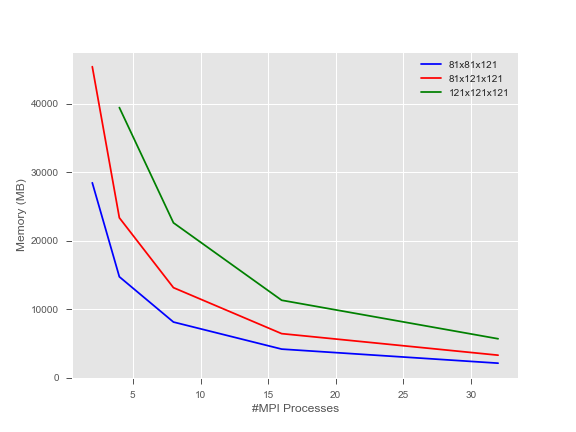
\includegraphics[width=\textwidth]{images/memoryMPI.png}
    \caption{Avg. Space in MBYTES per working proc for LU factorization on classical nodes }
    \label{memoryMPI}
  \end{subfigure}
  %
  \begin{subfigure}[b]{0.7\textwidth}
    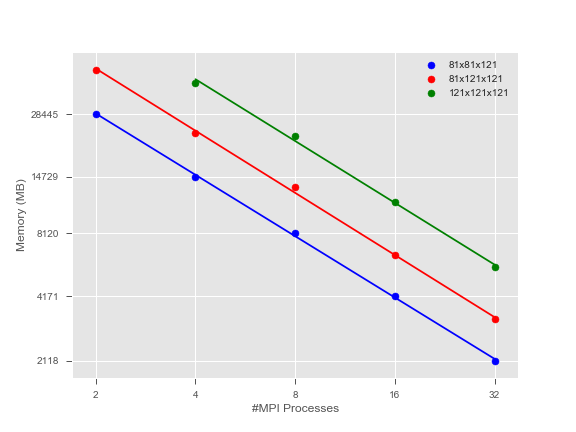
\includegraphics[width=\textwidth]{images/MemoryMPIlog.png}
    \caption{Avg. Space in MBYTES per working proc for LU factorization in log scale on classical nodes}
    \label{MemoryMPIlog}
  \end{subfigure}
\end{figure} 

\begin{figure}
\centering 
  \begin{subfigure}[b]{0.7\textwidth}
    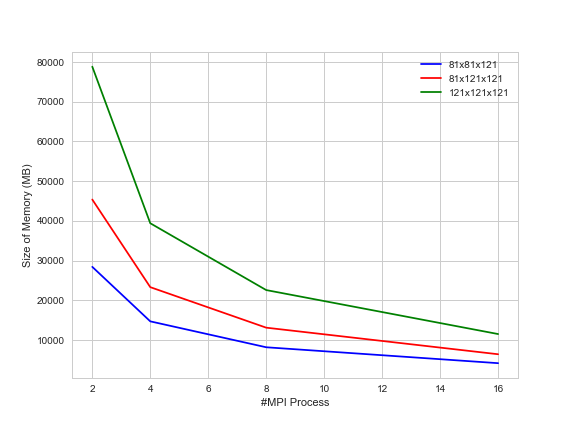
\includegraphics[width=\textwidth]{images/memoryMescaMPI.png}
    \caption{Avg. Space in MBYTES per working proc in LU factorization}
    \label{sim2}
  \end{subfigure}
  %
  \begin{subfigure}[b]{0.7\textwidth}
    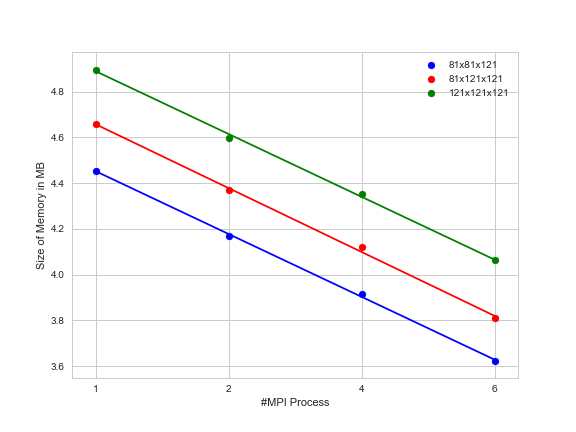
\includegraphics[width=\textwidth]{images/MemoryMescaMPIlog.png}
    \caption{Avg. Space in MBYTES per working proc in LU factorization in log scale}
    \label{sim3}
  \end{subfigure}
\end{figure} 

.............................. \newline
Comment ......................
.............................. \newline
\begin{figure}[]
\centering 
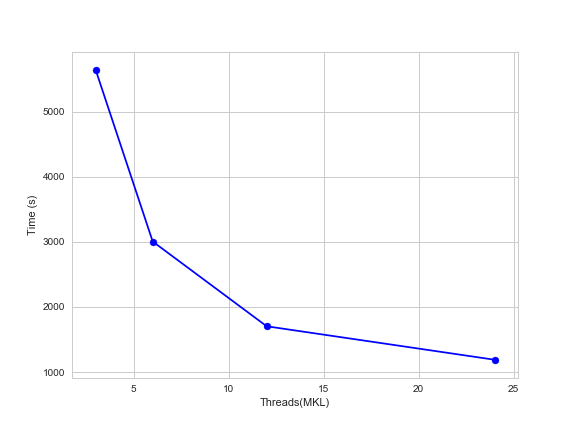
\includegraphics[width=0.75\textwidth]{images/TimeThreads.png}
\caption{Elapsed Time for LU factorization function of number of threads in Mesca node}
\label{Mesca_Time} 
\end{figure}

.............................. \newline
Comment ...................... 
.............................. \newline

\begin{figure}[]
\centering 
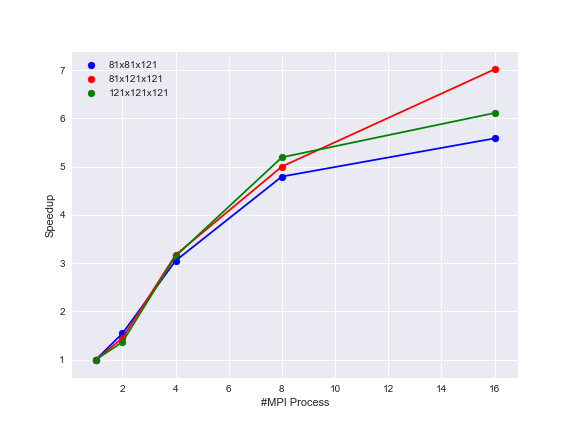
\includegraphics[width=0.75\textwidth]{images/SpeedupMesca.png}
\caption{Speedup in Mesca node}
\label{Mesca_Time} 
\end{figure}
\begin{figure}[]
\centering 
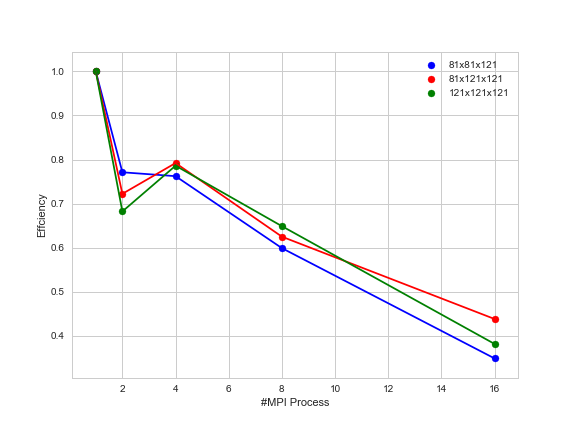
\includegraphics[width=0.75\textwidth]{images/EffciencyMesca.png}
\caption{Efficiency in Mesca node}
\label{Mesca_Time} 
\end{figure}



.............................. \newline
Comment ...................... \newline
.............................. \newline



\begin{figure}[]
\centering 
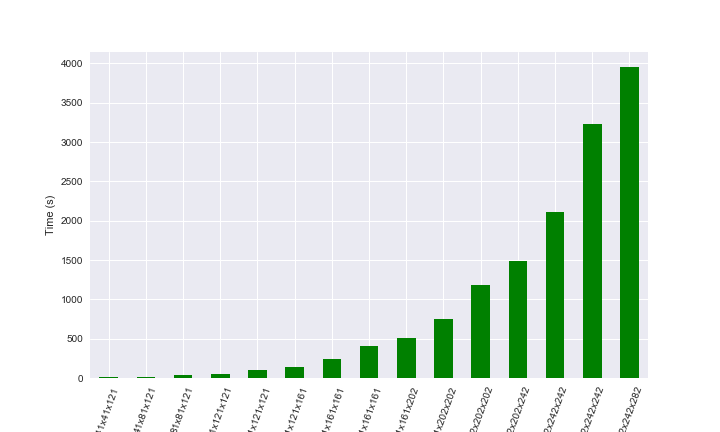
\includegraphics[width=0.75\textwidth]{images/Mesca_Time.png}
\caption{Time in LU factorization in Mesca node}
\label{Mesca_Time} 
\end{figure}
\begin{figure}[]
\centering 
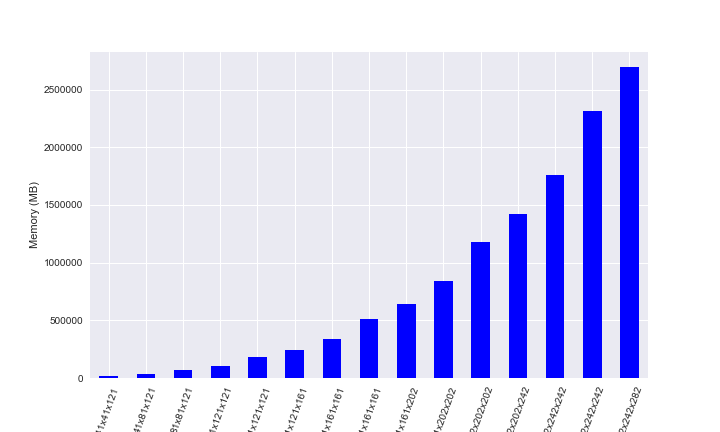
\includegraphics[width=0.75\textwidth]{images/Mesca_Memory.png}
\caption{Memory consumption in LU factorization in Mesca node}
\label{Mesca_Memory} 
\end{figure}
.............................. \newline
Comment ......................
.............................. \newline

Placement of Threads: KMP AFFINITY

\begin{table}[!h]
\centering

\label{Mesca1}
\begin{tabular}{lllllllllllll}
KMP\_AFFINITY & Grid dimensions & npml & \#MPI & \#th & \#Cores & $T_{LU}(s)$ &$Avg. Mem_{LU}/proc(MB)$ & $Mem_{LU}(MB)$ & $T(s)$ \\
 \hline
scatter &	$92 \times 181 \times 321; dz=50$ &	8 &	8 &	24 & 192 &	396.3693 & 73402 &	587218 & 7m39.295s \\
compact &	$92 \times 181 \times 321; dz=50$ &	8 & 8 &	24 & 192 &	435.1387 & 73402 &	587218 & 8m17.930s

\end{tabular}
\caption{Homogeneous Isotropic running on Mesca node}
\end{table}


.............................. \newline
Comment ......................
.............................. \newline

Case study: Ovethrust. \newline

\begin{table}[!h]
\centering

\label{amestoy}
\begin{tabular}{llllllllll}
Freq & Grid dimensions & npml &  & \#MPI & \#th & \#Cores & $T_{LU}(s)$  \\
 \hline
3.5, 4, 4.5, 5 & $ 66 \times 130 \times 230; dz=70$ & 8 & 24 & 10 & 240 & 78 \\
7 &	$ 92 \times 181 \times 321; dz=50 $ &	8 & 32 & 10	& 320 & 322 \\
10 & $ 131 \times 258 \times 458; dz=35$ &	4 &	68 & 10	& 680 &	1153

\end{tabular}
\caption{}
\end{table}

\begin{table}[!h]
\centering

\label{amestoyMesca}
\begin{tabular}{lllllllllll}
Freq & Grid dimensions & npml & \#MPI & \#th & \#Cores & $T_{LU}(s)$ & $ T(s)$ \\
 \hline
3	& $ 66 \times 130 \times 230; dz=70$ &	8 & 5 & 24	& 120 &	194.0989 & 3m42.937s  \\
3,5	& $ 66 \times 130 \times 230; dz=70$ &	8 &	8 &	15 &	120 &	98.9756 & 2m4.808s  \\
7	& $ 92 \times 181 \times 321; dz=50 $ & 8 & 8 & 20 &	160	& 439.0829 & 8m21.590s  \\
7	& $ 92\times 181 \times 321; dz=50 $ &	8 &	8 &	24 &	192	& 396.3693 & 7m39.295s	 \\							
10	& $ 131 \times 258 \times 458; dz=35$ &	4	& 8 &	24 & 192	 & 2182.6717 &	38m58.811s
\end{tabular}
\caption{}
\end{table}
\section{Profiling}
\section{Results} % Conclusion is usually a chapter itself.
%\chapter*{Discussion and Perspectives} 
% This is where we stop counting pages.
% Acknowledgements and References (and appendices) are not counted.
%-----------------------------------------------------------------------------
% Uncomment the next two lines if you have an appendix
% Appendices are usually not counted, and are only allowed if you
% speak to Barry about the need for it. Get approval first,
% and use this format. An appendix is not necessary for an
% essay's completeness.
%\appendix
%\renewcommand*{\theHchapter}{\Alph{chapter}}
%\chapter{The Title of Your First Appendix}
\label{ap: app1}
% We number appendices as in the main file, A, B, C.
% The appendice has title, do not include "Appendix" above.
% You need permission from Barry to have Appendices
% Why is it necessary? Does it add value?

Do you \textit{really} need an appendix? What does it add?

\section{section title}
Text text text text text text text text text text text text text text
text text text text text text text text text text text text text text. 

Rule 1 Rule 2 Rule 3. Everyone knows that.

%\endappendix
%-----------------------------------------------------------------------------
% See the acknowledgement.tex file and follow the instructions there.
\chapter*{Acknowledgements}
% Don't change anything above this.
% We do not number this or add it to the contents!
% Overly long acknowledgements are not professsional.

This is optional and should be at most half a page.
Thanks Ma, Thanks Pa. One paragraph in normal language is the most respectful.  

Do not use too much bold, any figures, or sign at the bottom. 
\chapter{The Title of Your First Appendix}
\label{ap: app1}
% We number appendices as in the main file, A, B, C.
% The appendice has title, do not include "Appendix" above.
% You need permission from Barry to have Appendices
% Why is it necessary? Does it add value?

Do you \textit{really} need an appendix? What does it add?

\section{section title}
Text text text text text text text text text text text text text text
text text text text text text text text text text text text text text. 

Rule 1 Rule 2 Rule 3. Everyone knows that.

%-----------------------------------------------------------------------------
% Note the errata page is not for now, it is for use during the examination.
% Not that you're going to have any errata.
%-----------------------------------------------------------------------------
% THE BIBLIOGRAPHY 
% Bibliography styles define how the bibliography is 
% listed and formatted.
% AMS alpha is a human-friendly bibliography style which
% we use by default here.  You are encouraged to use it.
% If your supervisor and tutor confirms that the field 
% you work in (physics, finance, etc.) generally use another
% style than amsalpha, then you may change to that style.
\renewcommand{\bibname}{References}
\nocite{*}
\bibliographystyle{amsalpha}
\bibliography{Senegal-Essay-Template}
\addcontentsline{toc}{chapter}{References}
%-----------------------------------------------------------------------------
\end{document}
